 \documentclass{MScthesisITEM}

% this package is just to generate text for demo-purposes

\usepackage{color}
\usepackage{parskip}
\usepackage{blindtext}
\usepackage{mathtools} % math packages
\usepackage{todonotes}
\usepackage{hyperref}
\usepackage{subcaption}
\usepackage{wrapfig}
\usepackage{pgfplots}
\usepackage{filecontents}
\usepackage{url}
\usepackage{float}
\usepackage{listings}
\usepackage{amsfonts}
\usepackage{amssymb}

\usepackage{float}
\usepackage{tikz}
\usetikzlibrary{positioning, fit, calc, shapes, arrows}
\usepackage{pgf-umlsd}
%\usepackage[procnames]{listings}

%\pgfplotsset{compat=1.11}
\setlength{\parindent}{0pt}

\definecolor{keywords}{RGB}{255,0,90}
\definecolor{comments}{RGB}{0,0,113}
\definecolor{red}{RGB}{160,0,0}
\definecolor{green}{RGB}{0,150,0}

\lstset{
	numbers=left,
	stepnumber=1, 
	numbersep=5pt,
	showspaces=false,
	showstringspaces=false,
	showtabs=false,
	basicstyle=\footnotesize, 
	numberstyle=\footnotesize, 
	tabsize=2, 
	breaklines=true,
	captionpos=b,}



\title{Identity-Based Trust Model in Named Data Networking} % The title of your assignement; NB use \newlinetitle to start a newline
\author{Haakon Garseg Mørk} % Your firstname and lastname
\professor{Stig F. Mjølsnes, ITEM} % Affiliation = ITEM for instance
\supervisor{N/A}

%% Uncomment the following in case you want subfigures; note that there will be a warning for the caption package
% \let\subcaption\undefined
% \let\subfloat\undefined
% \usepackage[bf]{caption}
% \usepackage{subcaption}

\DeclareGraphicsExtensions{.pdf,.jpg}
\graphicspath{{./figs/}}

\loadglsentries{glossary}
\makeglossaries

\begin{document}
\selectlanguage{english}
\pagenumbering{roman}
\pagestyle{plain}

%% Only for the project; comment out the line below for the master's thesis; the front page will be generated automatically by DAIM
%\titleITEM

%% Only for the master's thesis; for the project report the description is taken from It's Learning and added by the department
% \selectlanguage{english} % Change to 'norsk' if you are writing in Norwegian
% \begin{titlingpage}

\noindent
\begin{tabular}{@{}p{4cm}l}
\textbf{Title:} 	& Identity-Based Trust Model in Named Data Networking \\
\textbf{Student:}	& Haakon Garseg Mørk \\
\end{tabular}

\vspace{4ex}
\noindent\textbf{Problem description:}
\vspace{2ex}

The translation from name to address and location is a fundamental problem to all networks.
Named Data Networking (NDN) is a proposal for content-centric discovery and routing approach to networking
going on at the University of California, Los Angeles (UCLA) [1], which is part of the inspiration and a contact point for this work.

This project aims to understand the ideas and concepts of named data networking, and investigate the
potential these notions hold for network security, even for properties of anonymity and privacy. 
The student work should be to build a public key distribution application that uses ChronoSync [2] and runs over NDN.
This approach will allow for easy experimentation in the regular internet protocols environment.     

[1]  UCLA.  Named Data Networking. Web site at http://named-data.net/

[2]  UCLA, Named-data Networking. ChronoSync https://github.com/named-data/ChronoSync

\noindent
\begin{tabular}{@{}p{4cm}l}
\textbf{Responsible professor:} 	& Stig F. Mjølsnes \\
\textbf{Supervisor:}			& Stig F. Mjølsnes \\
\end{tabular}

\end{titlingpage}
% \cleardoublepage

%% There must be an abstract in English, even though the main text is in Norwegian
\selectlanguage{english}
\pagestyle{empty}
\begin{abstract}
Abstract goes here...
\end{abstract}
\cleardoublepage

%% Only for the master's thesis; if the main text is in English and you can write Norwegian, there must be an abstract in Norwegian as well.
% \selectlanguage{norsk}
% \pagestyle{empty}
\begin{abstract}

IP nettverket ble bygd for flere ti\r{a}r siden, og med dagens bruk av Internet ser vi at en ny nettverksprotokoll er s\r{a}rt trengt.
Named Data Networking (NDN) er en foresl\r{a}tt nettverksprotokoll som baserer seg p\r{a} innhold, istedenfor punkt-til-punkt arkitekturen som er grunnlaget for IP.
Selv med flere ti\r{a}rs bruk av Internet, er enn\r{a} ikke problemene med Public Key Infrastructure (PKI) l\o{}st. 
I NDN, har man heller ikke klart \r{a} finne en l\o{}sning p\r{a} dette.
Identitetsbasert kryptografi (IBC) viser seg \r{a} være anvendelig til tr\r{a}dl\o{}se sensornettverk, og enda mer n\r{a}r sensornettverket kj\o{}rer over NDN.

I denne masteroppgaven forklarer jeg NDN arkitekturen og de grunnlegende prinsippene i IBC.
Jeg modellerer og implementerer en applikasjon for \r{a} demonstrere bruken av IBC over NDN i et tenkt sensornettverk.

Implementasjonen og testingen av mitt bidrag verifiserer relevansen av IBC i et sensornettverk som kj\o{}rer over NDN, samt brukervennligheten rundt det \r{a} utvikle applikasjoner over NDN.

Jeg formelt og uformelt beviser sikkerheten i protokollene som er foresl\r{a}tt til enhetsregistrering og data foresp\o{}rsel i applikasjonen.

\end{abstract}
% \cleardoublepage

\selectlanguage{english}% Change to 'norsk' if you are writing in Norwegian

% \renewcommand{\abstractname}{Preface}
\begin{abstract}
\noindent \blindtext 
\end{abstract}
% \cleardoublepage

\renewcommand{\abstractname}{Acknowledgments}
\begin{abstract}
I am eternally grateful for the support of my fellow student, Eirik Auran Rathe.
Mr. Rathe has helped me with extraordinary suggestions, different approaches, and last but not least, his dick in my ass.

\end{abstract}
\cleardoublepage

% similarly you may add a separate acknowledgments page

\tableofcontents*
\cleardoublepage

%% include if relevant
\listoffigures
\cleardoublepage

\lstlistoflistings
\cleardoublepage

%% include if relevant
\listoftables
\cleardoublepage

%% include if relevant
%\listofalgorithms
%\addcontentsline{toc}{chapter}{List of Algorithms}
%\cleardoublepage

%% include if relevant
\printglossary[title=List of Terms, style=long]
\cleardoublepage
% \glsaddall[]

% include if relevant
\printglossary[title=List of Acronyms,type=\acronymtype] % prints just the list of acronyms
\cleardoublepage

\pagenumbering{arabic}
\pagestyle{ruled}
\chapter{Introduction}\label{chp:introduction} 

\section{Motivation}
The translation from name to address and location is a fundamental problem to all networks.
\gls{NDN} is a proposal for content-centric discovery and routing approach to networking
going on at the \gls{UCLA}, which is part of the inspiration and a contact point for this work.

In general, the name to address resolution can either be maintained by a catalogue lookup service, 
such as \gls{DNS} (Internet) and \gls{HLR} (mobile networks), 
or resolved on-the-fly by a protocol on request, such as \gls{ARP} (\gls{LAN}). 
There has been a tremendous amount of work done on the naming problem in distributed systems, 
some became big failures (e.g. X.500) others such as the web \gls{URL}s are very successful. 
Bringing things even further, the \gls{DOI} system is a \gls{URI} directed at the content/object itself rather than a location. 
Very much related to the name/address problem is the information security problem of efficient and practical public key distribution, 
which remain unsolved in practice, even though a significant number of digital certificate and verification protocols and schemes have been proposed, and systems tested over the last two decades. 
One notable and early theoretical proposal is Rivest and Lampson \gls{SDSI} proposal~\cite{rivest1996sdsi},
and subsequent work, that may be revisited for applicable to named data networking.

\section{Problem and Scope}

When designing a new network protocol for the future Internet, one of the most significant changes should be that it is designed for security.
Trust management plays a big part in security, and thus we cannot design trust management on known \gls{IP} failures such as X.500. 
\gls{PKI} is a tough challenge to solve and the solution is probably not the one or the other, but rather case specific.

I address the trust management issue in a though sensor device network, e.g. a health sensor network.
By using the \gls{NFD} I will implement my proposal for such a sensor network.

\section{Methodology}

First I find in what context the Public Key System can be applicable, then I design the application flow in sequence diagrams.
Based on how \gls{NDN} is designed, I try to implement the proposed design and see where to redesign the application proposal for achieving minimal communication overhead, security (i.e. \gls{CIA}) and usability.

\section{Outline}

This paper will first introduce one of the proposed protocols for the future Internet, \gls{NDN}.
I will explain the architecture of \gls{NDN} as well as some related work regarding my application proposal. 
The application modules will be explain in detail and implementation choices will be discussed.
At last I will present the results of the implementation and my conclusion of the trust model.
\chapter{Background}\label{chp:background} 
Ingress


\section{Information-Centric networking}\label{chp2:sec:icn}
\gls{ICN} ...


\section{NDN Architecture}\label{chp2:sec:ndn_architecture}
\gls{NDN} ...

\subsection{Naming}
Naming is left to the application design.
\chapter{Identity-Based Cryptography}\label{chp:ibc}
This chapter will present the concept of \gls{IBE} and \gls{IBS}, and why it is highly applicable to use this type of cryptography in \gls{NDN}. 
The possibilities to use the file synchronization module to do key distribution and revocation will be introduced.

\section{Notations}
Notations related to \gls{IBC} used throughout this thesis is listed in~\autoref{tbl:notations}.
\begin{table}[h]
  \begin{tabular}[c]{p{0.5\textwidth}p{0.5\textwidth}}
  \hline
  Symbol                    & Description                               \\ \hline
  MPK\textsubscript{i}      & Master Public Key belonging to i          \\ %\hline
  MSK\textsubscript{i}      & Master Secret Key belonging to i          \\ %\hline
  SK\textsubscript{i}       & Secret Key (private key) belonging to i   \\ %\hline
  PK\textsubscript{i}       & Public Key belonging to i                 \\ %\hline
  ID\textsubscript{i}       & Identity belonging to i                   \\ %\hline
  \end{tabular}
  \caption[IBC Notations]{IBC notations used throughout the thesis.}
  \label{tbl:notations}
\end{table}

\section{Concept}\label{ibc}
\gls{IBE} was first proposed by Shamir~\cite{DBLP:conf/crypto/Shamir84} in 1984. 
Shamir proposed a scheme for \gls{IBS}, but not a scheme for \gls{IBE}. 
The concept of \gls{IBE} builds upon every user having an \gls{ID} that is used as the \gls{PK}. 
This \gls{ID} can be anything, i.e. email, phone number, \gls{SSN}, or a \gls{name} (\autoref{name}).
The \gls{SK} that is extracted from the \gls{ID} is issued by a \gls{TTP}.
Notice that if every user could have created their own \gls{SK}, then so could anybody else with the same computational power, since the user does not obtain any ``privileged'' information about its \gls{ID}~\cite{Bidgoli06}.
This eliminates the need of certificates because the \gls{SK} allocation itself is a verfication by the \gls{TTP}.
The \gls{IBE} implementation remained unsolved until 2001, when Dan Boneh and Matthew K. Franklin proposed~\cite{DBLP:conf/crypto/BonehF01}.
However the scheme has only been shown to be secure within the random oracles model~\cite{DBLP:journals/iacr/Waters04}, hence less practical.

\gls{IBE} is based on performing asymmetric encryption with a publicly know \gls{ID} working as the \gls{PK}.
As seen in~\autoref{eq:mapping-id-name-pk}, the \gls{ID} can be a \gls{name} (e.g. ``/ndn/no/ntnu/haakon'').
Hence the \gls{name} becomes the \gls{PK} (from now referred to as \gls{ID}).
Therefore \gls{IBE} is highly applicable to \gls{NDN}.

\begin{equation}\label{eq:mapping-id-name-pk}
ID_{device} = PK_{device} = Name_{device}
\end{equation}

In \gls{IBE} there is a \gls{TTP} that is called \gls{PKG}.
The \gls{PKG}s task is to extract a \gls{SK} given an \gls{ID} and provide public parameters (\gls{MPK}) needed for performing encryption, decryption, signing and verifying. In~\autoref{fig:pkg_functions} the \gls{IBC} methods is illustrated in practice. 
\autoref{eq:keypair-id-sk} shows the key pair \gls{ID} and \gls{SK} which is used in \gls{IBC}.
\begin{equation}\label{eq:keypair-id-sk}
(ID_{device}, SK_{device})
\end{equation}
First the \texttt{PKG} runs \texttt{Setup()}. 
\texttt{device1} can then request a \texttt{SK} by sending \texttt{ID\textsubscript{d1}} to the \texttt{PKG}. 
In return the \texttt{device1} receives the \texttt{SK\textsubscript{d1}} as well as the \texttt{MPK\textsubscript{PKG}}.
\texttt{device2}, which is already a part of the trust domain, sends a signed request for \gls{data} to \texttt{device1}. 
\texttt{device1} verifies the signature and responds to the request with a signed, encrypted content.
\texttt{device0}, which do not have a \gls{SK} generated from the \texttt{PKG} and thus is not a part of the trust domain, sends a request to \texttt{device1} that is declined.

\begin{enumerate}\label{ibc-methods}
  \item \texttt{Setup()} generates the key pair \texttt{(\gls{MPK}, \gls{MSK})}. 
  These keys are used by only the \gls{PKG} to extracting secret keys, encryption and decryption.
  \item \texttt{Extract(MPK\textsubscript{PKG}, MSK\textsubscript{PKG}, ID\textsubscript{device})} generates a secret key from a given ID. 
  \item \texttt{Encrypt(MPK\textsubscript{PKG}, ID\textsubscript{device}, message)} encrypts the message.
  \item \texttt{Decrypt(MPK\textsubscript{PKG}, SK\textsubscript{device}, cipher)} decrypts the cipher generated from the encryption.
  \item \texttt{Sign(MPK\textsubscript{PKG}, SK\textsubscript{device}, message)} signs a hash digest of the message (e.g. \gls{SHA1}).
  \item \texttt{Verify(MPK\textsubscript{PKG}, ID\textsubscript{device}, message, signature)} verifies the signature.
\end{enumerate}

\begin{figure}[ht]
  \centering
  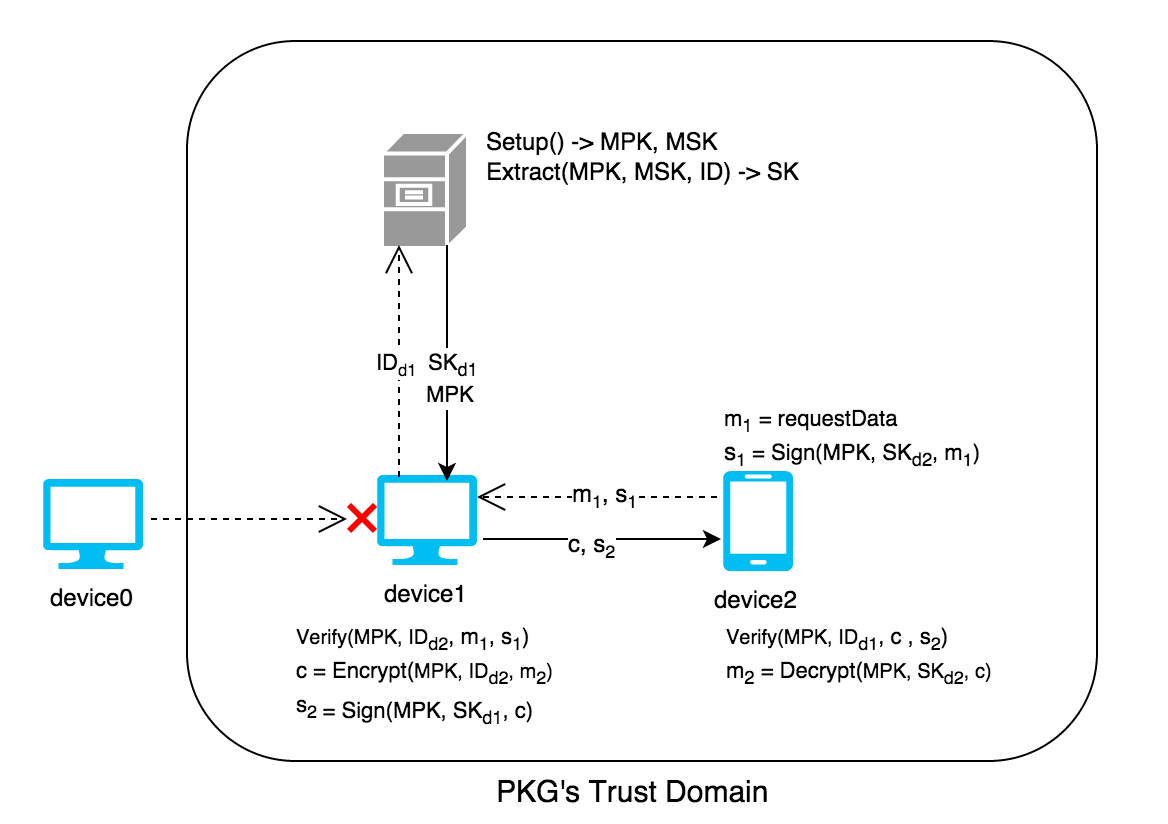
\includegraphics[width=1\textwidth]{pkg_functions.png}
  \caption[IBC methods]{Methods of an IBC systems illustrated in practice.
  The PKG calls \texttt{Setup()} which generates the key pair \texttt{(MPK, MSK)}.
  Device1 then requests registration by sending its ID\textsubscript{d1} to the PKG.
  PKG extracts the SK\textsubscript{d1} composing the key pair \texttt{(ID\textsubscript{d1}, SK\textsubscript{d1})}.
  After retrieving the SK\textsubscript{d1}, device1 receives an request for a resource, signed by another device in the trust domain.
  The request is verified and the resource requested is encrypted and sent as a response.
  Finally, device2 verifies the response and decrypts the resource content.
  Device0 requests the same resource, but the request is denied because the verification fails, due to its inadequate signature.}
  \label{fig:pkg_functions}
\end{figure}

To encrypt a message with \gls{IBE}, the user encrypts a \gls{CEK} with the recipients \gls{ID}.
The user encrypts the message using the \gls{CEK} together with symmetric encryption~\cite[section 2.2.2]{rfc5408}, and sends both the encrypted \gls{CEK} and the encrypted content to the requester. 

It is two main concepts which holds a great part of the security in an \gls{IBC} system.
The security of \gls{IBC} depends mainly on the secrecy of the \gls{PKG}, therefor it is crucial to deploy a secure \gls{PKG}.
Also, it is important to identify each device before issuing \gls{SK}.
Approving wrong devices and allocating \gls{SK} to an adversary would compromize the system.

There are some drawbacks related to \gls{IBE} such as issues around trusting the \gls{PKG} considering that the \gls{PKG} generates all \gls{SK}s.  
If the \gls{PKG} is compromised by an adversary, the adversary will retrieve all \gls{SK}s belonging to the corresponding \gls{ID}. 
Suspicion of \gls{MITM}, where the \gls{PKG} is the adversary, can be a problem for users.
The same issue does however occur in Kerberos, which is a well recognized security system.
Initializing might also be a problem because to allocate \gls{SK}s, a secure channel has to be established. 
However, this is not a bugger problem than in existing networks. 
Pre-shared secrets or Diffie-Hellman key exchange might be a good solution.

\section{Security}\label{ibe-secureness}
When designing protocols in cryptography one first usually designs an ideal system where all parties have random oracle access, then proves the security.
A random oracle is like a ``black box'' that outputs truly random numbers.
Second, one replaces the oracle access with a hash function.
This gives an implementation of an ideal system in the real world, but without random oracles~\cite{DBLP:conf/ccs/BellareR93}. 
It is perfectly fine to make statements based on the ideal system, but debatable whether the same statements yields for the implementation in the real world.
Canetti et al. concluded that there exist secure schemes in the \textit{Random Oracle Model}, but for which any implementation of the random oracle results in insecure schemes~\cite{DBLP:journals/jacm/CanettiGH04}.
Boneh and Franklins \gls{IBE} scheme is only secure when using random oracles, and relies on elliptic curves~\cite{DBLP:conf/crypto/BonehF01}.

Following the \textit{Standard Model} one does not resort to the random oracle heuristic and does not rely on non-standard complexity assumptions.
Hence proving security in the standard model is preferably.
In 2004 Boneh and Boyen proposed a fully secure scheme in the standard model~\cite{DBLP:conf/crypto/BonehB04}.
However the scheme is not efficient. 

The complexity assumptions is based on bilinear maps.
Let $\mathbb{G}_1$ and $\mathbb{G}_2$ be groups of prime order \gls{p}, and $g$ be a generator of \gls{g}. 
We say that $\mathbb{G}$ has a bilinear map $e : \mathbb{G}_1 \times \mathbb{G}_2 \to \mathbb{G}_T$ if $e$ is efficiently computable, $e$ is bilinear, i.e. $e(g^a, g^b) = e(g, g)^{ab}$ (for all $a$ and $b$), and $e$ is non-degenerate, i.e. $e(g,g)\neq 1$.
For more details about bilinear maps and~\gls{BDH} used in \gls{IBE}, the reader is encouraged to take a look at~\cite{DBLP:conf/crypto/BonehF01,DBLP:journals/iacr/Naccache05}.

First practical scheme was introduces by Brent Waters~\cite{DBLP:journals/iacr/Waters04}.
But as David Naccache states in his paper~\cite{DBLP:journals/iacr/Naccache05}, Waters' scheme without random oracles introduces too large public parameters (164\gls{KB}!).
Naccache proves that he was able to construct a practical and fully secure scheme in the standard model based on the \gls{DBDH} assumption.
The scheme is a modification of Waters' scheme, but with public parameters of just a few \gls{KB} size.

Waters created a fully secure \gls{IBE} system with short parameters under \gls{simple_assumption} in 2009~\cite{DBLP:conf/crypto/Waters09}.




\chapter{Key Infrastructure}
This chapter will present the concept of \gls{IBE} and \gls{IBS}, and why it is highly applicable to use this type of cryptography in \gls{NDN}. 
Then the possibilities to use the file synchronization module to do key distribution and revocation will be introduced.

\section{Identity-Based Cryptography}\label{ibc}
\gls{IBE} was first proposed by Shamir~\cite{DBLP:conf/crypto/Shamir84} in 1984. 
The concept of \gls{IBE} builds upon every user having an \gls{ID} that is used as the public key. 
This \gls{ID} can be anything, i.e. email, phone number, \gls{SSN}, or a Name (~\autoref{name}).
This eliminates the need of certificates.
Shamir did propose a scheme for \gls{IBS}, but not a scheme for \gls{IBE}. 
The \gls{IBE} implementation remained unsolved until 2001, when Dan Boneh and Matthew K. Franklin proposed~\cite{DBLP:conf/crypto/BonehF01}.
However the scheme has only been shown to be secure with a random oracles model~\cite{DBLP:journals/iacr/Waters04}, hence less practical.


\gls{IBE} is based upon performing cryptography with a publicly know \gls{ID}.
Since the \gls{ID} can be practically anything it is highly applicable for \gls{NDN} where the \gls{ID} can be a Name (``/ndn/no/ntnu/haakon'').
Hence the Name becomes the public key. 

There is a \gls{TTP} in \gls{IBE} that is called \gls{PKG}.
The \gls{PKG}s task is to produce a private key that corresponds to a given ID and provide 

\begin{enumerate}\label{ibc-methods}
  \item \texttt{Setup()} generates a key pair, \gls{MPK} and \gls{MSK}. These keys are used by only the \gls{PKG} to extracting private keys, encryption and decryption.
  \item \texttt{Extract(MPK, MSK, ID)} generates a Private Key from a given ID. 
  \item \texttt{Encrypt(MPK, ID, message)} encrypts the message.
  \item \texttt{Decrypt(MPK, private key, cipher)} decrypts the cipher generated from the encryption.
  \item \texttt{Signing(MPK, private key, message)} signs a hash digest of the message (e.g. \gls{SHA1}).
  \item \texttt{Verify(MPK, ID, message, signature)} verifies the signature.
\end{enumerate}

\begin{figure}[ht]
  \centering
  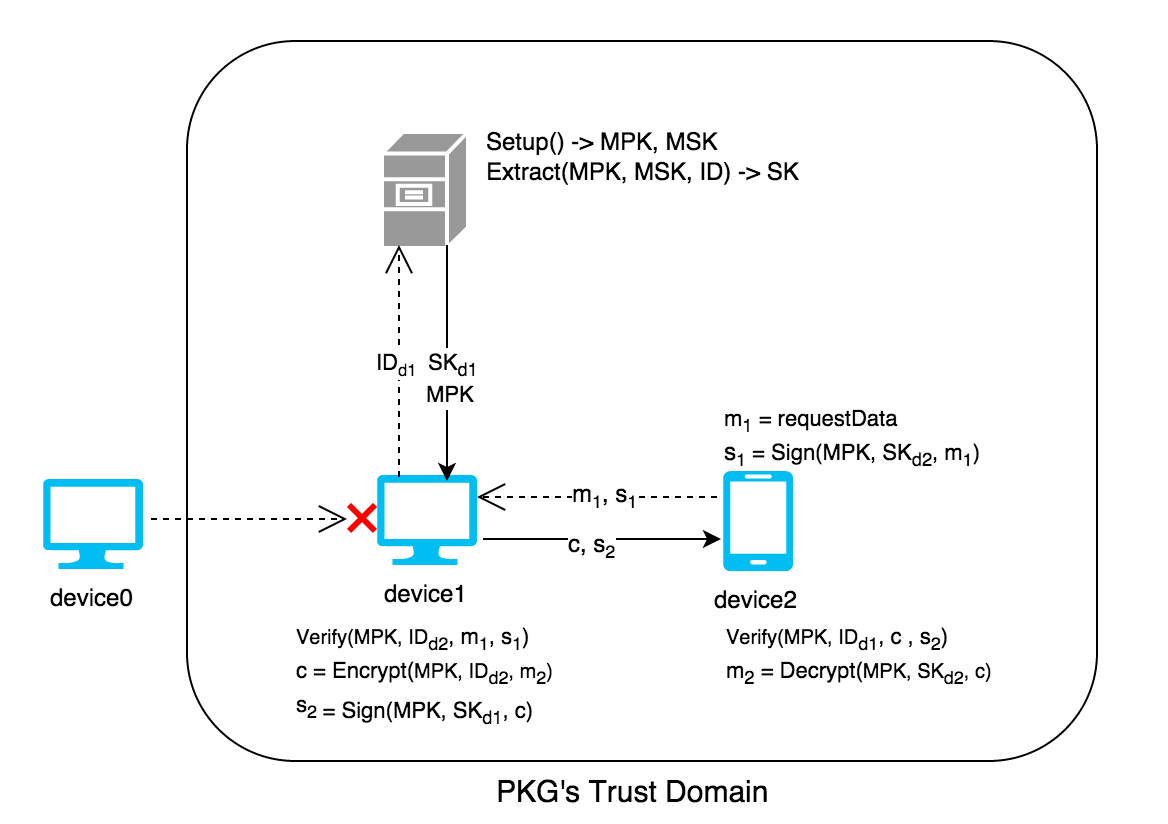
\includegraphics[width=1\textwidth]{pkg_functions.png}
  \caption{Methods of an IBC systems illustrated in action.}
  \label{fig:pkg_functions}
\end{figure}

To encrypt a message with \gls{IBE}, the user encrypts a \gls{CEK} with the recipients \gls{ID}.
The user encrypts the message using the \gls{CEK} together with symmetric encryption~\cite[section 2.2.2]{rfc5408}, and sends both the encrypted \gls{CEK} and the encrypted content to the requester. 

Some drawbacks related to \gls{IBE} are listed below:
\begin{enumerate}
	\item If \gls{PKG} is compromised. Adversary has private key to all nodes that used the compromised \gls{PKG}
	\item \gls{PKG} can read and write messages related to the node, because it has all private keys, i.e. \gls{MITM}.
	\item \gls{PKG} and the requesting node has to establish a secure channel. 
\end{enumerate}

\section{Identity-Based Cryptography - Secureness}

A random oracle is like a ``black box'' that outputs truly random numbers.
When designing protocols in cryptography one first usually designs an ideal system where all parties have random oracle access, then proves the security.
Second, one replaces the oracle access with a hash function.
This gives an implementation of an ideal system in the real world, but without random oracles~\cite{DBLP:conf/ccs/BellareR93}. 
It is just fine to make statements based on the ideal system, but debatable whether the same statements yields for the implementation in the real world.
Canetti et al. concluded that there exist secure schemes in the \textit{Random Oracle Model}, but for which any implementation of the random oracle results in insecure schemes~\cite{DBLP:journals/jacm/CanettiGH04}.
Boneh and Franklins \gls{IBE} scheme is only secure when using random oracles.

Following the \textit{Standard Model} one does not resort to the random oracle heuristic and does not rely on non-standard complexity assumptions.
Hence proving security in the standard model is preferably.
In 2014 Boneh and Boyen proposed a fully secure scheme in the standard model~\cite{DBLP:conf/crypto/BonehB04}.
However it is not efficient. 

First practical scheme was ~\cite{DBLP:journals/iacr/Waters04}.
But as David Naccache states in his paper~\cite{DBLP:journals/iacr/Naccache05}, Waters' scheme without random oracles introduces too large public parameters (164\gls{KB}!).
Naccache proves that he was able to construct a practical and fully secure scheme in the standard model based on the \gls{DBDH} assumption.
The scheme is a modification of Waters' scheme, but with public parameters of just a few \gls{KB} size.

Brent Waters created a fully secure \gls{IBE} system with short parameters under simple assumption in 2009~\cite{DBLP:conf/crypto/Waters09}.

To understand the mathematical assumptions for \gls{IBE}, the reader should take a look at~\cite[section 3]{DBLP:conf/crypto/BonehF01} for details about bilinear maps and~\gls{BDH}.

\section{Key Distribution}
Instead of in \gls{PKI} where each public key is signed by a certificate authority and the generated certificate is sent as a response in \gls{HTTPS} then validated by the the client, I want to make the certificate authority obsolete by distributing every \gls{ID} (public key) issued by the \gls{PKG}.
This can be done through an IDSync application built upon the application presented in~\autoref{file-sync}.
In~\autoref{fig:pkg_sync} we see that the \gls{PKG} multicasts the \gls{ID} list to all devices that have joined the domain.
Each device can verify the integrity and authenticity of the sync state Data and be sure that the \gls{ID} list surely originates from its own \gls{PKG}.
\begin{figure}[ht]
  \centering
  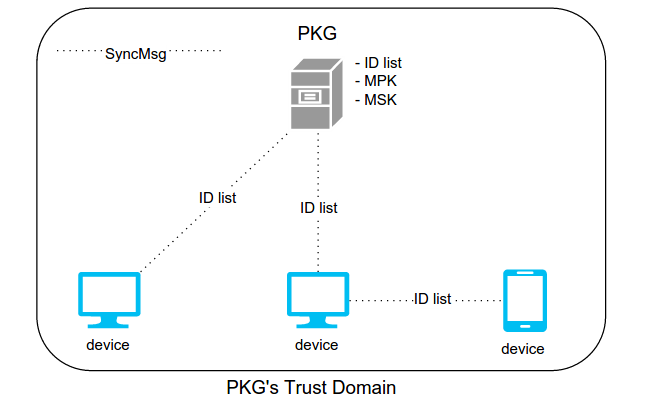
\includegraphics[width=1\textwidth]{pkg_sync.png}
  \caption{IDSync with tree devices and a PKG.}
  \label{fig:pkg_sync}
\end{figure}

\section{Key Revocation}
Few alternatives to revocation scheme in \gls{IBE}.
Key Revocation in IBE ~\cite{DBLP:journals/iacr/BoldyrevaGK12} 
One suggestion is to allocate private keys with the public key combined with some sort of date, e.g. month-year or just year. 
In this alternative a user has to renew its private key each time the date changes, i.e. either the month or the year depending on the date format.
The problem with the revocation solution is that it is cumbersome for the \gls{PKG}.


Key revocation becomes obsolete with the IDSync distribution solution. 

\chapter{Sensor Application}\label{sensor-application}
In this chapter the sensor application will be presented. 
Several sequence diagrams will be explained, as well as concepts needed to understand the flow of the application. 

\section{Health Sensors}
There is an ongoing discussion of when the health technology revolution will come to human bodies now that \gls{IoT} have become so popular.
By revolution, I mean sensors placed in the human body. 
Sensors that can read your blood pressure, heart rate and measure insulin levels.
Sensors that can detect whether your body is missing a substance, or if it is poisoned. 
There is no limit for what can be done.
Everything that should be measured, will be measured by sensors integrated in the human body.
But who will be able to read the \gls{data}?
Or perform instructions to the sensors/devices?
There is some major privacy issues related to this discussion, and problems that needs to be solved.

In 2011, Jerome Radcliffe discovered that his insulin pump easily could be hacked~\cite{radcliffe2011hacking}.
Basically the pump would take instructions from anyone and do anything, with no questions asked. 
This is a worst case scenario when it comes to hacking medical devices attached to a human.

For this matter I propose a \gls{HSS} that is built upon \gls{NDN} with \gls{IBC} ensuring a secure and locked environment.
First, let me introduce you to The Stig. 
He has developed diabetes and he does not want to manually monitor his glucose levels and adjust the insulin pump every meal. 
He has injected a \gls{CGM} to monitor his glucose levels and report to the insulin pump, automatically.
In addition to his diabetes, he has a heart disease which forces him to monitor his heart rate at any given time. 
In~\autoref{fig:health-sensor-system} we can see The Stig with all his sensors and devices. 
The \gls{CGM} reports periodically to the insulin pump, and all sensors reports to The Stig's mobile so that The Stig can watch what is going on.

\begin{figure}[ht]
  \centering
  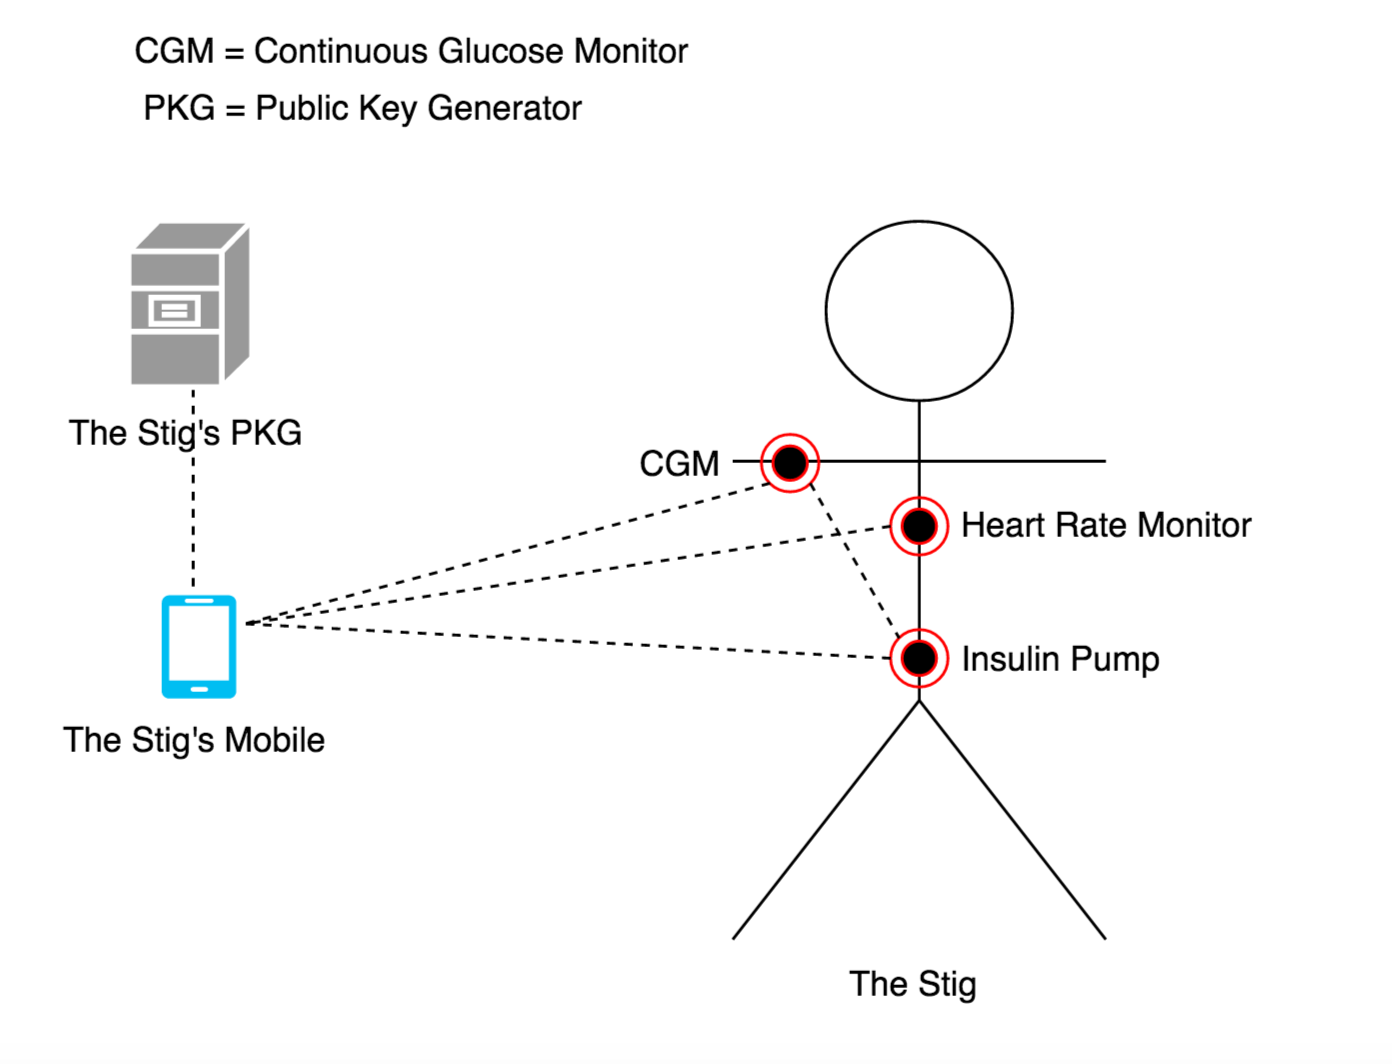
\includegraphics[width=1\textwidth]{health-sensor-system.png}
  \caption{Health Sensor System}
  \label{fig:health-sensor-system}
\end{figure}

\section{Health Sensor System}\label{hss}
To have a secure system, it needs to be established trust between the sensors and the devices.
There need to be integrity controls, confidentiality protection and access control. 
In the following sections, I will describe the protocols suggested for achieving the mentioned goals.

\subsection{Rendezvous Authentication}\label{rendezvous_authentication}
One of the best solutions for authentication of an identity in cryptography is rendezvous authentication, the concept of meeting face-to-face for authenticating who you are talking to. 
Most cases in \gls{IoT} we have the advantage of identifying devices in a physical manner.
This means that it is possible to authenticate devices, such as sensors. 
Typically, this kind of authentication will rely on 1) manually inspection and 2) digital connection, e.g. through \gls{NFC}.
In the proposed system, I assume that this type of authentication is achieved in a secure manner and do not discuss how this should be done.
Typically this kind of authenticated connection should be used to preload a secret key to devices, establishing authentication in a later phase.
% Also there is the concept of human-computer authentication~\cite{DBLP:journals/iacr/GilbertRS05, DBLP:conf/crypto/JuelsW05, DBLP:conf/percom/Weis05}.
% This authentication method uses a shared secret before authentication. 

\subsection{System Initialization Phase}
When The Stig is setting up his \gls{HSS}, first he have to configure the \gls{PKG}. 
Any type of computer can play the role of the \gls{PKG} and The Stig has chosen his home server, from now ``the PKG''.
The Stig is now the only admin user in the system, hence he has full control over which device that should be granted access to the trust domain.
The \gls{PKG} runs the \texttt{Setup()} which creates key pairs that is used to do \gls{IBE} and \gls{IBS}.
Second, he wants his mobile device, from now ``the mobile'', to be a part of the \gls{PKG}s trust domain, and further add all of the other devices and sensors, from now ``device(s)''. 
This is done through a device registration phase.

\subsection{Device Registration Phase}\label{init}
The goal for the device registration protocol is to achieve a secure one-round secret key exchange.
For the protocol to be secure, there are several issues that need to be addressed. 
1) The response message containing the secret key has to be encrypted. 
This can be achieved by using a pre-shared symmetric key to do encryption on the \gls{SK}.
2) The response message has to be signed by the \gls{PKG} for integrity and authenticity reasons.
3) A nonce have to be present for replay protection.
The pre-shared symmetric key should be a temporary random generated key. 
Thus the device registration \gls{interest} between the device and the \gls{PKG} can be unique.
This implies that the device can authenticate itself in a way that an adversary cannot do.

The device registration is divided into two phases. 
Phase 1 is the sharing of a temporary random key \texttt{tk} used to secure phase 2, illustrated in~\autoref{fig:init_ibe_1}.
Phase 2 is the \gls{SK} allocation, illustrated in~\autoref{fig:init_ibe_2}.

\textit{Phase 1}.
Trust is difficult to be established without a rendezvous authentication or any form of pre-established trust chain like e.g. a certificate chain.
I do not assume that every device is a part of such trust chain before registration, and thus the trust between the device and the \gls{PKG} have to be based on the concept explained in~\autoref{rendezvous_authentication}, with manually inspection of the device and preloading of a temporary random key \texttt{tk}.
The packet flow of the key preloading, done over e.g. \gls{NFC}, is shown in~\autoref{fig:init_ibe_1}.
The device generates a temporary random key \texttt{tk} and together with the ID\textsubscript{d}, are loaded onto the \gls{PKG}.
The device receives the ID\textsubscript{PKG} and the MPK\textsubscript{PKG} in return.
Since $ID_{PKG} = Name_{PKG}$, the device now what \gls{Name} the \texttt{Init} \gls{interest} should have.
It can also verify signatures from the \gls{PKG}, with the MPK\textsubscript{PKG}. 
Before phase 2, an admin user have to approve the requesting ID\textsubscript{d} and the corresponding \texttt{tk}.

\begin{figure}[ht]
  \centering
  \begin{tikzpicture}[node distance=6cm,auto,>=stealth']
      \node[] (server) {pkg};
      \node[left = of server] (client) {device};
      \node[below of=server, node distance=4cm] (server_ground) {};
      \node[below of=client, node distance=4cm] (client_ground) {};
      %
      \draw (client) -- (client_ground);
      \draw (server) -- (server_ground);
      
      \draw ($(client)!0.15!(client_ground)$) 
      -- node[above,scale=0.8,right]{ID\textsubscript{d}, tk} 
      ($(client)!0.15!(client_ground)$);
      \draw ($(server)!0.15!(server_ground)$) 
      -- node[above,scale=0.8,right]{(msk, mpk), (ID\textsubscript{pkg}, sk\textsubscript{pkg})} 
      ($(server)!0.15!(server_ground)$);
      
      \draw[->] ($(client)!0.45!(client_ground)$) 
      -- node[above,scale=0.8,midway]{ID\textsubscript{d} || tk} 
      ($(server)!0.45!(server_ground)$);
      \draw[<-] ($(client)!0.65!(client_ground)$) 
      -- node[above,scale=0.8,midway]{ID\textsubscript{pkg} || mpk} 
      ($(server)!0.65!(server_ground)$);
      \draw ($(server)!0.80!(server_ground)$) 
      -- node[above,scale=0.8,right]{Admin manually approves ID\textsubscript{d}} 
      ($(server)!0.80!(server_ground)$);
  \end{tikzpicture}
  \caption{Device Registration, phase 1.
  The messages are exchanged through e.g. NFC (\autoref{rendezvous_authentication}), and thus are protected against any adversaries outside the range of the NFC signal (\textasciitilde{1} meter).
  At first the Device generates a temporary random key \texttt{tk} and sends this key and its \texttt{ID\textsubscript{d}} to the PKG. 
  The PKG responds with its \texttt{ID\textsubscript{PKG}} and finally an admin user have to approve the requesting device. 
  }
  \label{fig:init_ibe_1}
\end{figure}

\textit{Phase 2}.
Now that both the device and the \gls{PKG} possesses the shared secret \texttt{tk} and the device have been approved by an admin user, the phase 2 can begin.
The device sends an \texttt{Init} \gls{interest} that contains its ID\textsubscript{d} and a nonce which is encrypted with the \texttt{tk}.
The \gls{PKG} decrypts the message and uses the received ID to extract the \gls{SK} for the device (this will be the key belonging to the \gls{PKG}s trust domain) and uses the \texttt{tk} to do symmetric \gls{AES} encryption on the secret key. 
The \gls{data} response to the \texttt{Init} \gls{interest} will contain the encrypted \gls{SK}, the nonce and a signature.
To finish the device registration protocol, the device decrypts the secret key, checks the nonce and verify that the \gls{SK} allocated actually belongs to the earlier received \gls{MPK} and that is corresponds to its \gls{ID}.
The device has established a trust with its \gls{PKG} and can verify other devices within this trust domain. 

\begin{figure}[ht]
  \centering
  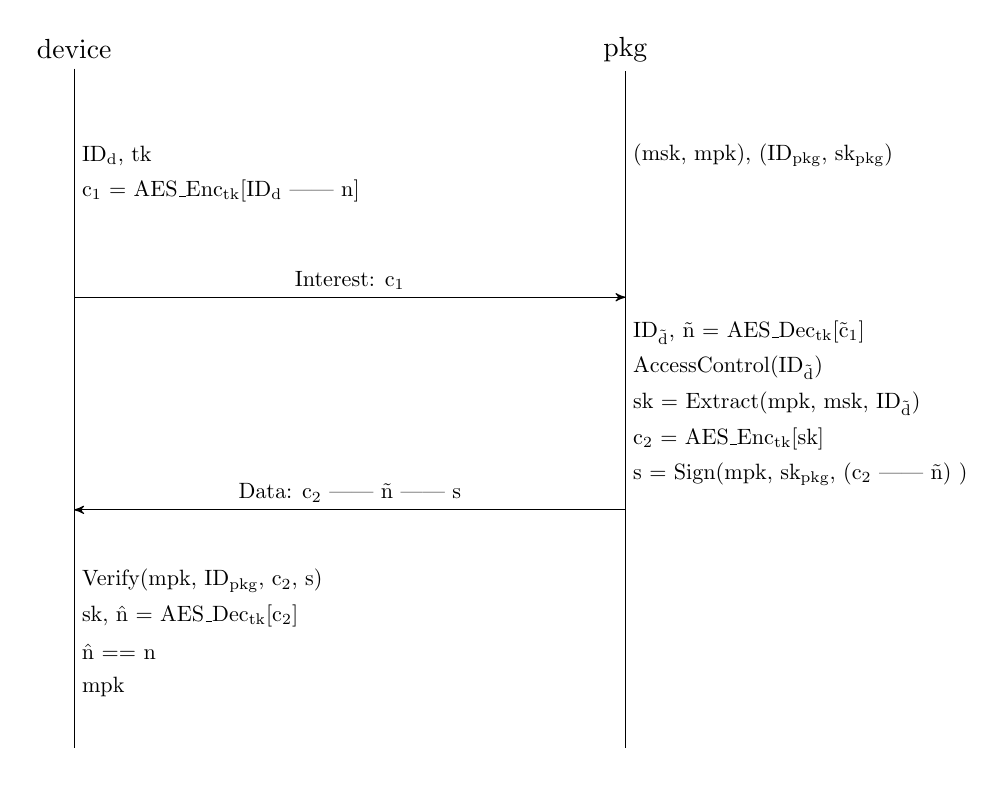
\begin{tikzpicture}[node distance=6cm,auto,>=stealth']
      \node[] (server) {pkg};
      \node[left = of server] (client) {device};
      \node[below of=server, node distance=9cm] (server_ground) {};
      \node[below of=client, node distance=9cm] (client_ground) {};
      %
      \draw (client) -- (client_ground);
      \draw (server) -- (server_ground);

      \draw ($(client)!0.15!(client_ground)$) 
      -- node[above,scale=0.8,right]{ID\textsubscript{d}, tk} 
      ($(client)!0.15!(client_ground)$);
      \draw ($(server)!0.15!(server_ground)$) 
      -- node[above,scale=0.8,right]{(msk, mpk), (ID\textsubscript{pkg}, sk\textsubscript{pkg})} 
      ($(server)!0.15!(server_ground)$);

      \draw ($(client)!0.20!(client_ground)$) 
      -- node[above,scale=0.8,right]{c\textsubscript{1} = AES\_Enc\textsubscript{tk}[ID\textsubscript{d} || n] } 
      ($(client)!0.20!(client_ground)$);
      \draw[->] ($(client)!0.35!(client_ground)$) 
      -- node[above,scale=0.8,midway]{Interest: c\textsubscript{1}} 
      ($(server)!0.35!(server_ground)$);
      \draw ($(server)!0.40!(server_ground)$) 
      -- node[above,scale=0.8,right]{ID\textsubscript{\~{d}}, \~{n} = AES\_Dec\textsubscript{tk}[\~{c}\textsubscript{1}] } 
      ($(server)!0.40!(server_ground)$);
      \draw ($(server)!0.45!(server_ground)$) 
      -- node[above,scale=0.8,right]{AccessControl(ID\textsubscript{\~{d}}) } 
      ($(server)!0.45!(server_ground)$);
      \draw ($(server)!0.50!(server_ground)$) 
      -- node[above,scale=0.8,right]{sk = Extract(mpk, msk, ID\textsubscript{\~{d}}) } 
      ($(server)!0.50!(server_ground)$);
      \draw ($(server)!0.55!(server_ground)$) 
      -- node[above,scale=0.8,right]{c\textsubscript{2} = AES\_Enc\textsubscript{tk}[sk] } 
      ($(server)!0.55!(server_ground)$);
      \draw ($(server)!0.60!(server_ground)$) 
      -- node[above,scale=0.8,right]{s = Sign(mpk, sk\textsubscript{pkg}, (c\textsubscript{2} || \~{n}) ) } 
      ($(server)!0.60!(server_ground)$);
      

      \draw[<-] ($(client)!0.65!(client_ground)$) 
      -- node[above,scale=0.8,midway]{Data: c\textsubscript{2} || \~{n} || s} 
      ($(server)!0.65!(server_ground)$);
      \draw ($(client)!0.75!(client_ground)$) 
      -- node[above,scale=0.8,right]{Verify(mpk, ID\textsubscript{pkg}, c\textsubscript{2}, s) } 
      ($(client)!0.75!(client_ground)$);
      \draw ($(client)!0.80!(client_ground)$) 
      -- node[above,scale=0.8,right]{sk, \^{n} = AES\_Dec\textsubscript{tk}[c\textsubscript{2}] } 
      ($(client)!0.80!(client_ground)$);
      \draw ($(client)!0.85!(client_ground)$) 
      -- node[above,scale=0.8,right]{\^{n} == n } 
      ($(client)!0.85!(client_ground)$);
      \draw ($(client)!0.90!(client_ground)$) 
      -- node[above,scale=0.8,right]{mpk} 
      ($(client)!0.90!(client_ground)$);
  \end{tikzpicture}
  \caption{Device Registration, phase 2. 
  The device sends a Init Interest encrypting nonce \texttt{n} and its \texttt{ID\textsubscript{d}}.
  The device receives the response, decrypts the cipher \texttt{c\textsubscript{1}}, checks if the \texttt{ID\textsubscript{d}} is approved, extracts the secret key corresponding to \texttt{ID\textsubscript{d}}, encrypts the secret key and finally signs the Data.
  }
  \label{fig:init_ibe_2}
\end{figure}


% \begin{figure}[ht]
%   \centering
%   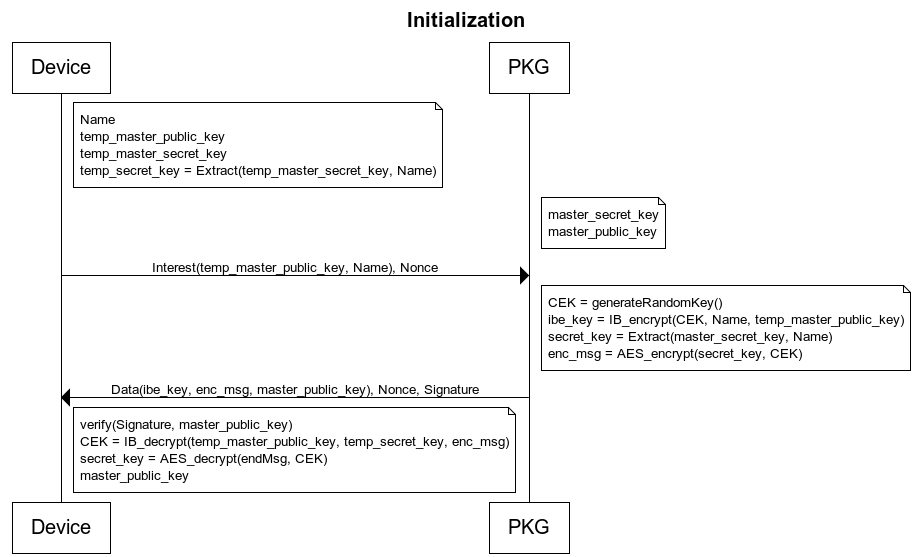
\includegraphics[width=1\textwidth]{Initialization.png}
%   \caption{Initialization IBE}
%   \label{fig:init_ibe_1}
% \end{figure}

Now that the mobile is authenticated, devices can connect to the mobile through e.g. \gls{NFC} for initialization.
This results in a rendezvous authentication between the device and the mobile, and if the mobile is given the authorities to perform initialization (\autoref{access_control}), the new device can join the \gls{PKG}s trust domain.

\subsubsection{Security Analysis}
It is important that the protocol possesses privacy, availability and control properties. 
I shortly present a formal security analysis by modeling the protocol in \gls{spdl} and verifying certain claims through Scyther~\cite{DBLP:conf/cav/Cremers08}.
After that, an informal discussion of the security in the protocol will be presented.

\textit{Scyther}.
The analysis proves that the protocol is confidential, replay and injection resistant, and possesses integrity and authenticity.
All claims made (i.e. \texttt{alive}, \texttt{secret}, \texttt{weakagree}, \texttt{niagree}, \texttt{nisynch}) shows no attacks in Scyther.
The \gls{spdl} code of the protocol can be reviewed in~\autoref{apx:scyther-analysis-dr}.

\textit{Authenticity}.
The protocol holds the required authenticity and integrity. 
The pre-shared temporary random key \texttt{tk} is shared in an assumed secure manner, thus appending an encrypted message to the Init Interest, is used as an authentication for the \gls{PKG}.
Thus the encryption, with the \texttt{tk} as key, protects against \gls{MITM} attacks.
The response \gls{data} is hashed and signed with the \gls{PKG}s \gls{SK} which provides authenticity and integrity for the requesting device.
The signature can easily be verified, and since an adversary do not obtain a polynomial time algorithm that can forge the \gls{SK} the device can be sure that the message is signed by the corresponding ID, which is the ID\textsubscript{PKG} received in the device registration phase 1, seen in~\autoref{fig:init_ibe_1}.
Thus the signature protects against \gls{MITM} attacks.

\textit{Confidentiality}. 
The \gls{SK} will be encrypted with the pre-shared temporary random key \texttt{tk}, and thus the confidentiality is preserved.
An adversary will only be able to know the \gls{MPK}, cipher texts, signatures and both IDs, which is not required to be confidential and not sufficient to compute the \gls{SK} that is extracted. 
The adversary do not obtain a polynomial time algorithm that can compute the \gls{SK} from the known parameters.
Hence an adversary have to obtain a algorithm to compute the secret keys, which is the same polynomial time algorithm as in the sub section above that the adversary do not have access to.

\textit{Replay}.
Since the adversary cannot compute \texttt{tk} nor forge the signature, it cannot send \gls{interest} nor \gls{data} that is captured at any arbitrary point. 
Devices keep track of the nonce corresponding to a data pull, hence a replay with will be detected and thrown away.

\subsection{Deployment Phase}\label{data_pull}
The goal for this protocol is to achieve a secure one-round data pull with authorization and integrity.
For the protocol to work and the data pull to be successful, 1) both devices has to belong to the same trust domain (i.e. has initialized with the same \gls{PKG}) and 2) the requester has to have granted access rights for the resource requested.

As illustrated in~\autoref{fig:health-sensor-system}, the device has joined the \gls{PKG}s trust domain and is ready to communicate with other devices.
This flow is illustrated in~\autoref{fig:data_pull_ibe}.
First the requester has to express an \gls{interest} to the target device asking for a specific resource. 
The \gls{receiver} checks whether the requester has access rights to the requested resource and verifies that the requester is a part of the same trust domain.
If the \gls{receiver} is authorized, the \gls{receiver} responds with the \gls{data} containing the resource. 
The requester signs the \gls{interest} and appends it to the content \gls{name}.
The \gls{receiver} will also do a symmetric encryption on the sensor \gls{data} and do a asymmetric encryption on the \gls{CEK} with the requester's \gls{ID}.
This step is only performed if \gls{data} confidentiality is needed. 
Then the \gls{data} packet is signed and sent.
Finally the requester receives the \gls{data}, verifies the signature and decrypts the sensor \gls{data}.

\begin{figure}[ht]
  \centering
  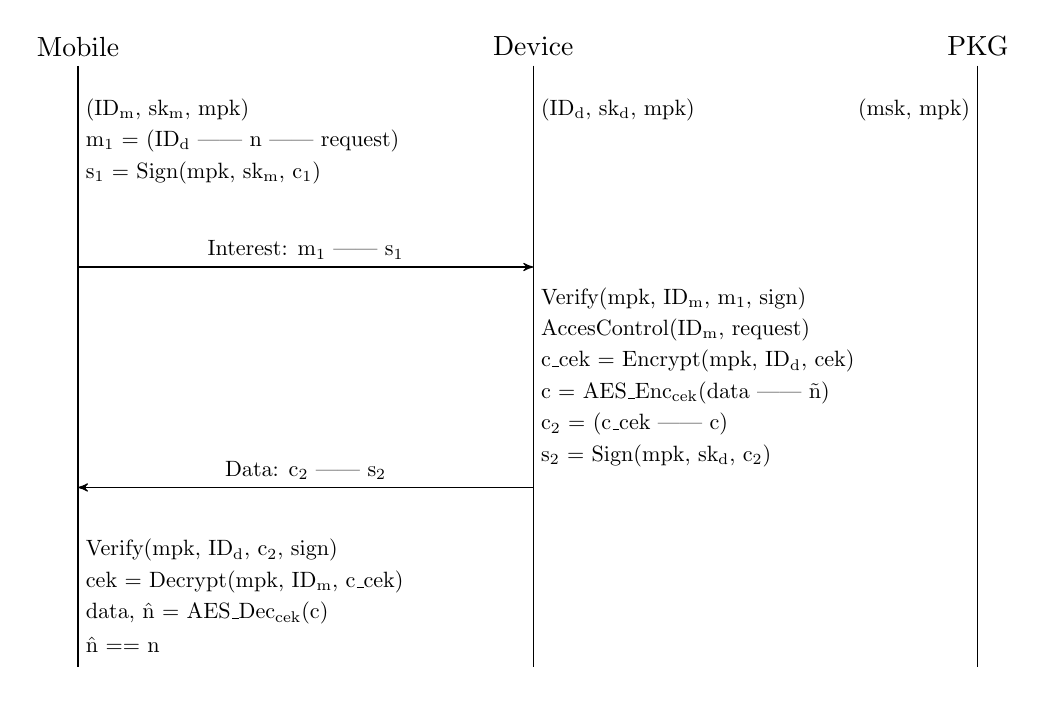
\begin{tikzpicture}[node distance=4.5cm,auto,>=stealth']
      \node[] (server) {PKG};
      \node[left = of server] (client_1) {Device};
      \node[left = of client_1] (client_0) {Mobile};
      \node[below of=server, node distance=8cm] (server_ground) {};
      \node[below of=client_0, node distance=8cm] (client_0_ground) {};
      \node[below of=client_1, node distance=8cm] (client_1_ground) {};
      %
      
      \draw (server) -- (server_ground);
      \draw (client_0) -- (client_0_ground);
      \draw (client_1) -- (client_1_ground);
      
      \draw ($(client_0)!0.10!(client_0_ground)$) 
      -- node[above,scale=0.8,right]{(ID\textsubscript{m}, sk\textsubscript{m}, mpk)} 
      ($(client_0)!0.10!(client_0_ground)$);
      \draw ($(client_1)!0.10!(client_1_ground)$) 
      -- node[above,scale=0.8,right]{(ID\textsubscript{d}, sk\textsubscript{d}, mpk)} 
      ($(client_1)!0.10!(client_1_ground)$);
      \draw ($(server)!0.10!(server_ground)$) 
      -- node[above,scale=0.8,left]{(msk, mpk)} 
      ($(server)!0.10!(server_ground)$);


      \draw ($(client_0)!0.15!(client_0_ground)$) 
      -- node[above,scale=0.8,right]{m\textsubscript{1} = (ID\textsubscript{d} || n || request)} 
      ($(client_0)!0.15!(client_0_ground)$);
      \draw ($(client_0)!0.20!(client_0_ground)$) 
      -- node[above,scale=0.8,right]{s\textsubscript{1} = Sign(mpk, sk\textsubscript{m}, c\textsubscript{1})} 
      ($(client_0)!0.20!(client_0_ground)$);
      \draw[->] ($(client_0)!0.35!(client_0_ground)$) 
      -- node[above,scale=0.8,midway]{Interest: m\textsubscript{1} || s\textsubscript{1}} 
      ($(client_1)!0.35!(client_1_ground)$);
      \draw ($(client_1)!0.40!(client_1_ground)$) 
      -- node[above,scale=0.8,right]{Verify(mpk, ID\textsubscript{m}, m\textsubscript{1}, sign)} 
      ($(client_1)!0.40!(client_1_ground)$);
      \draw ($(client_1)!0.45!(client_1_ground)$) 
      -- node[above,scale=0.8,right]{AccesControl(ID\textsubscript{m}, request)} 
      ($(client_1)!0.45!(client_1_ground)$);
      \draw ($(client_1)!0.50!(client_1_ground)$) 
      -- node[above,scale=0.8,right]{c\_cek = Encrypt(mpk, ID\textsubscript{d}, cek)} 
      ($(client_1)!0.50!(client_1_ground)$);
      \draw ($(client_1)!0.55!(client_1_ground)$) 
      -- node[above,scale=0.8,right]{c = AES\_Enc\textsubscript{cek}(data || \~{n})} 
      ($(client_1)!0.55!(client_1_ground)$);
      \draw ($(client_1)!0.60!(client_1_ground)$) 
      -- node[above,scale=0.8,right]{c\textsubscript{2} = (c\_cek || c)} 
      ($(client_1)!0.60!(client_1_ground)$);
      \draw ($(client_1)!0.65!(client_1_ground)$) 
      -- node[above,scale=0.8,right]{s\textsubscript{2} = Sign(mpk, sk\textsubscript{d}, c\textsubscript{2})} 
      ($(client_1)!0.65!(client_1_ground)$);
      \draw[<-] ($(client_0)!0.70!(client_0_ground)$) 
      -- node[above,scale=0.8,midway]{Data: c\textsubscript{2} || s\textsubscript{2}} 
      ($(client_1)!0.70!(client_1_ground)$);

      \draw ($(client_0)!0.80!(client_0_ground)$) 
      -- node[above,scale=0.8,right]{Verify(mpk, ID\textsubscript{d}, c\textsubscript{2}, sign)} 
      ($(client_0)!0.80!(client_0_ground)$);
      \draw ($(client_0)!0.85!(client_0_ground)$) 
      -- node[above,scale=0.8,right]{cek = Decrypt(mpk, ID\textsubscript{m}, c\_cek)}
      ($(client_0)!0.85!(client_0_ground)$);
      \draw ($(client_0)!0.90!(client_0_ground)$) 
      -- node[above,scale=0.8,right]{data, \^{n} = AES\_Dec\textsubscript{cek}(c)} 
      ($(client_0)!0.90!(client_0_ground)$);
      \draw ($(client_0)!0.95!(client_0_ground)$) 
      -- node[above,scale=0.8,right]{\^{n} == n} 
      ($(client_0)!0.95!(client_0_ground)$);
  \end{tikzpicture}
  \caption{Data pull under deployment. 
  The mobile sends a Sensor Interest to the device appending the request for a resource and a nonce \texttt{n}. 
  The Interest is signed with the mobile's secret key \texttt{sk\textsubscript{m}} and verified by the device. 
  The device checks whether the mobile has a valid capability for the requested resource and encrypts the data if granted.
  The Data response is signed with the device's secret key \texttt{sk\textsubscript{d}}.
  The mobile decrypts of the content encryption key \texttt{cek} and the cipher \texttt{c}, checks whether the received nonce \texttt{\^{n}} is equal to \texttt{n} and finally accepts the data as correct.}
  \label{fig:data_pull_ibe}
\end{figure}

% \begin{figure}[ht]
%   \centering
%   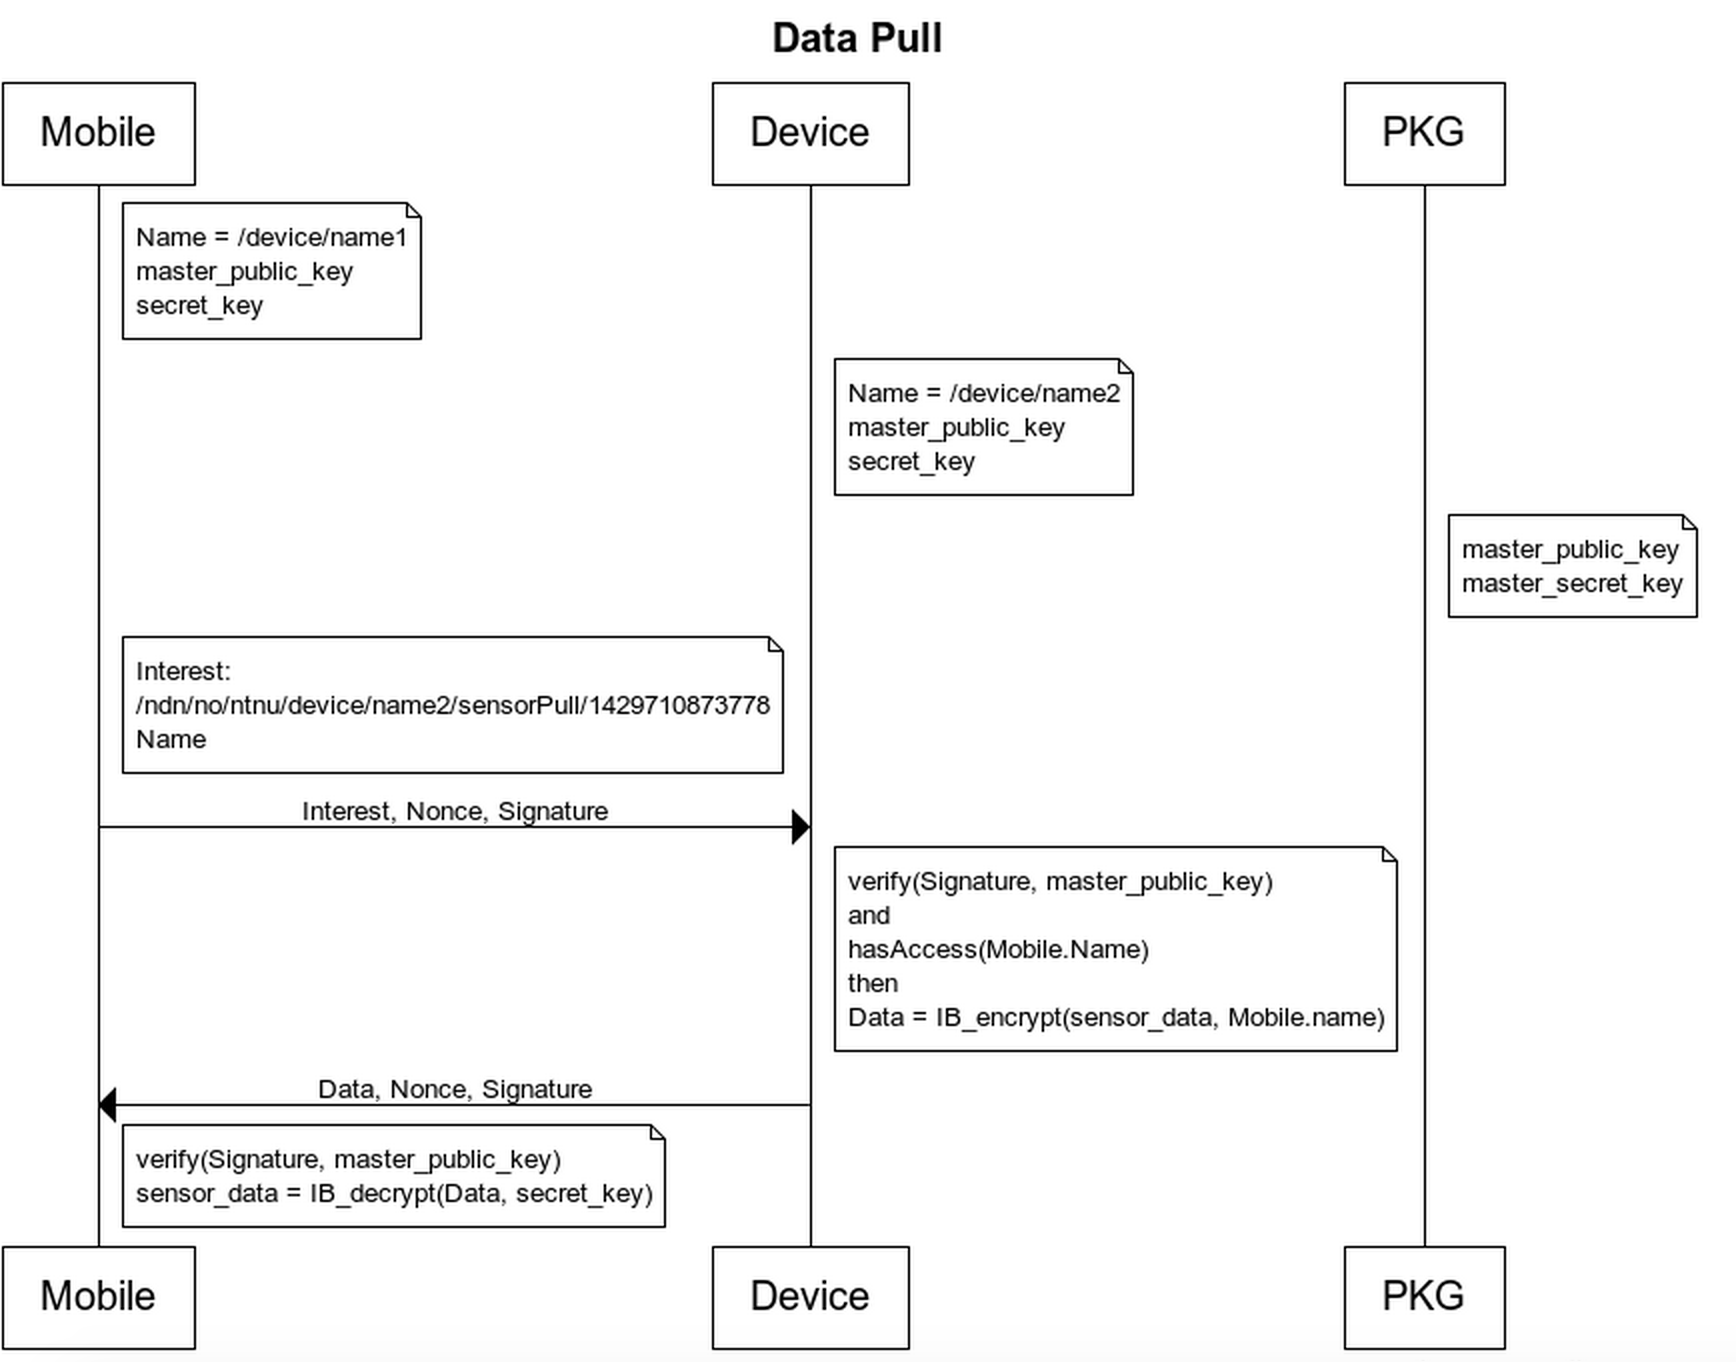
\includegraphics[width=1\textwidth]{DataPull.png}
%   \caption{Mobile performing a data pull from a device in the network.}
%   \label{fig:data_pull_ibe}
% \end{figure}

\subsubsection{Security Analysis}
It is important that the protocol possesses privacy, availability and control properties. 
I shortly present a formal security analysis by modeling the protocol in \gls{spdl} and verifying certain claims through Scyther.
After that, an informal discussion of the security in the protocol will be presented.

\textit{Scyther}.
The analysis proves that the protocol is confidential, replay and injection resistant, and possesses integrity and authenticity.
All claims made (i.e. \texttt{alive}, \texttt{secret}, \texttt{weakagree}, \texttt{niagree}, \texttt{nisynch}) shows no attacks in Scyther. 
The \gls{spdl} code of the protocol can be reviewed in~\autoref{apx:scyther-analysis-dp}.

\textit{Authenticity}.
The protocol holds the required authenticity and integrity. 
The message is hashed and signed with the senders \gls{SK} which provides authenticity and integrity.
The signature can easily be verified by the receiver, and since an adversary do not obtain a polynomial time algorithm that can forge the \gls{SK} one can be sure that the message is signed by the corresponding ID.
Thus the signature protects against \gls{MITM} attacks.

\textit{Confidentiality}. 
All \gls{data} that flows through the \gls{HSS} can be encrypted if necessary. 
When a resource is requested, the \gls{publisher} will do an access control to decide whether the ID\textsubscript{requester} has the right capabilities. 
The \gls{CEK} will be asymmetrically encrypted, and the resource data will be symmetrically encrypted, thus both key and data is confidential and only available to whoever has the corresponding \gls{SK} to the ID\textsubscript{requester}.
An adversary will only be able to know the \gls{MPK}, nonce, request, cipher and both IDs, which is not required to be confidential and not sufficient to compute the resource data. 
The adversary do not obtain a polynomial time algorithm that can compute the resource data from the known parameters.
Hence an adversary have to obtain a algorithm to compute the secret keys, which is the same polynomial time algorithm as in the sub section above that the adversary do not have access to.

\textit{Replay}.
Since the adversary cannot forge the signature, it cannot send \gls{interest} nor \gls{data} that is captured at any arbitrary point. 
This is due to the nonce presence in all packets. 
Devices keep track of the nonce corresponding to a data pull, hence a replay with will be detected and thrown away.

\subsection{Key Distribution using File Synchronization Module}

The Stig wants to have full control over the devices that are a part of the trust domain, and be able to remove a device if necessary.
Each device should have an updated list of all public keys, i.e. every devices' \gls{ID}.
The distribution of this list can easily be achieved by using the \gls{FSM} (\autoref{file-sync} \& \autoref{key-distribution}).
The \gls{PKG} will be the distributor in this synchronization and each device will be a subscriber.


\section{Informal Security Analysis}
In this section an informal security analysis of the whole system is presented.
The assumed threat model will first be presented, along with access control, \gls{CIA}, and trust model.

\subsection{Threat Model}
Threats that I find relevant for the \gls{HSS} can be categorized into three main categories: threats to privacy, threats to availability and threats to control.
I assume the following threat model:
\begin{enumerate}
  \item An adversary might try to eavesdrop information (privacy).
  \item An adversary might try to send bogus commands, e.g. injection, replay and \gls{MITM} (control).
  \item Jamming, node compromise (such as theft of mobile) and \gls{DoS} (availability).
\end{enumerate}

I assume that the \gls{PKG} cannot be compromised by any adversary, and thus the \gls{MSK} will always be hidden from any adversaries. 
However, it is extremely important that the machine which plays the role of the \gls{PKG} is secured in a physical matter, as well as remote secureness. 
The \gls{PKG} is the single point of failure in the whole system.

An idea introduced by Aaditeshwar Seth and Srinivasan Keshav in~\cite[Section 5.4]{Seth:2005:PSD:1897159.1897165} is to avoid storing the \gls{SK}s in devices that is more likely to be lost or stolen, e.g. a mobile.
Using \gls{HIBC}, one can extend the key hierarchy by another level that is time-based.
These time-based keys can then be downloaded to the mobile on a daily basis, hence the time the mobile will be compromised is reduced.

\subsection{Access Control}\label{access_control}
Since the ID\textsubscript{device} is appended to the \gls{interest} and the \gls{interest} is signed by the corresponding SK\textsubscript{device}, the \gls{ID} of the device can easily be authenticated. 
When a device retrieves an \gls{interest} for its sensor \gls{data}, there should be an authorization mechanism. 
One can argue that once a device has been authenticated in the \gls{PKG}s trust domain, everyone in the domain can be sure that the device will not abuse the information or functionalities available. 
However, due to scalability this is not a secure way to handle access control. 
If a device does not need a privilege, it does not need it.
Hence it should not have it. 
That is the least privilege access principle, which is default in Capability Based Approach to \gls{IoT} Access Control~\cite{DBLP:conf/imis/GusmeroliPR12}.
This approach has some additional benefits for the \gls{HSS}, such as

\begin{itemize}
  \item delegation support - 
  A device can grant access rights to other devices, as well as granting the right to further delegate these rights to a third device.
  \item capability revocation - 
  If the \gls{PKG} have granted delegation rights to a mobile, and the mobile is not found trustworthy after a while, the capabilities issued by the mobile can easily be revoked.
  \item information granularity - 
  Specific resources from a device can be granted access to in different granularity.
\end{itemize}

Another solution can be an \gls{ACL} based approach equivalent to what Wentao Shang et al. did in~\cite{DBLP:journals/network/ShangDMBZ14}.

\subsection{Confidentiality}
The confidentiality is achieved by doing asymmetric encryption on a \gls{CEK} that is used for symmetric encryption on the content.
As explained in the sequence diagram (\autoref{fig:data_pull_ibe}) presented in the above sections, each \gls{interest} appends the requester's ID (\autoref{eq:mapping-id-name-pk}).
Since the ID\textsubscript{requester} always is appended it can always be used to do asymmetric encryption, hence all \gls{CEK}s can be encrypted only for the requesting device, and thus the confidentiality in the system can always be achieved.

\subsection{Integrity and Authenticity}
Each device will obtain a secret key allocated by its superior \gls{PKG}, as explained in~\autoref{ibc}.
With the concept from~\autoref{rendezvous_authentication} together with the \gls{PKG}s \gls{MPK}, you can trust that the device is authorized for the \gls{PKG}s trust domain. 
Hence all signed packets can be verified by anyone with the \gls{MPK}.
In this setting, a verified signature acts as an assurance of authentication and integrity. 

Every \gls{interest} has a timestamp attached to the \gls{name} (e.g. \path{/ndn/no/ntnu/device/name2/sensorPull/1429710873778}), i.e. milliseconds from \texttt{UTC} \texttt{1970-01-01} \texttt{00:00:00}, that can be used for protection against replay attack. 

\subsection{Availability}
This is a harder problem to solve.
The network is purely wireless, hence vulnerable to jamming. 
An adversary could try to send infinite \gls{interest}s to a device with an invalid signature, hence the device may be overloaded with work and might run out of battery fast.
Therefore one should check the \gls{MPK} before doing any crypto.
This is also why I have chosen to append the MPK in the packet~\autoref{fig:sensor_interest-data}. 

\subsection{Trust Model}
For a system to be secure, cryptography together with trust is essential. 
The \gls{HSS} trust model is built upon trusting a centralized authority, typically the user's home server, rendezvous authentication and \gls{IBC}.
The fact that it runs over \gls{NDN} makes it easier to achieve security goals and usability for third party developers.

The \gls{PK} is the \gls{name} of the device, and all content published by the device will begin with this \gls{name}, hence it is easy to verify that the \gls{publisher} is the owner of the content.
To be able to verify and encrypt messages, the device need the MPK\textsubscript{PKG} and the ID of the user it wants to communicate with. 
If allowed by the PKG, the public parameters MPK\textsubscript{PKG} is public for everybody that is not a part of the trust domain. 
To be able to sign and decrypt messages the device have to be a member of the trust domain and be issued a secret key mapping to the ID\textsubscript{device}.
Each device builds its trust on other devices based on that it has been verified by an administrator that controls the \gls{PKG}.

\chapter{Implementation and Testing}
This chapter will first introduce the most significant frameworks that must be installed to be able to run \gls{NDN} applications.
Then the various designs and implementation choices will be explained.
The source code is left out from the appendix due to the size inconvenience. 
Finally, the test result will be presented.

\section{Installing Named Data Networking Protocol}

There are several libraries that is required for experimenting in a \gls{NDN} environment.
Installation guides can be found at the Github project~\cite{ndn-git}.
First we need to install the \gls{ndn-cxx}.
\gls{ndn-cxx} is a implementation of \gls{NDN} primitives. 
It is a fundamental framework that \gls{NDN} application requires. 
Second we need to install the \gls{NFD}~\cite{nfd} which is a network forwarder and also in the core implementation of \gls{NDN}.
The major modules implemented in \gls{NFD} is:
\begin{itemize}
  \item Core - Common services shared between the different \gls{NFD} modules (such as hash, \gls{DNS} resolver, face monitoring etc.).
  \item Faces - Generalization of different interfaces, explained in~\autoref{ndn-node-modules}.
  \item Tables - \gls{PIT}, \gls{CS}, \gls{FIB}, explained in~\autoref{ndn-node-modules}.
  \item Forwarding - Packet processing.
  \item Management - Enables users/programs to interact with the \gls{NFD} forwarder state.
  \item\gls{RIB} Management - Managing routing protocols and application prefix registration.
\end{itemize}
The \gls{NDN} project is under development, and thus the implementation of \gls{NFD} has its deficiencies.
Ideally we want the devices to communicate directly with each other using WiFi, without running over \gls{IP}. 
This face functionality is not yet implemented, and thus \gls{NDN} is running over \gls{IP} in my experiments.

\subsection{Installing PyNDN2}
The work done in this thesis is written in Python, hence the \gls{PyNDN2}~\cite{pyndn2-git} is used.
This is an easy to use implementation of \gls{NDN} and comes with great code examples.

Because the \gls{NDN} protocol require signing of \gls{data} packets (\autoref{ndn-security}) some new implementation in the \gls{PyNDN2} source code was necessary to be able to sign and verify with \gls{IBS}.
I added the \path{python/pyndn/sha256_with_ibswaters_signature.py} file that follows the pattern of the existing RSA Signature (\path{python/pyndn/sha256_with_rsa_signature.py}) and is of type \texttt{Signature}.
Some small additions in the \path{python/pyndn/encoding/tlv_0_1_1_wire_format.py} and the \path{python/pyndn/encoding/tlv/tlv.py} is added so \gls{PyNDN2} recognizes the \gls{IBS} when the \gls{data} packet is encoded and decoded.

\section{Installing Identity-Based Cryptography}
To be able to run \gls{IBC} the \gls{PBC}~\cite{ben2007implementation} needs to be installed.
I use the Charm framework~\cite{charm13} implements several \gls{IBE} and \gls{IBS} schemes in Python.
Charm is a framework for rapidly prototyping cryptosystems.


Some small modifications had to be done in the Waters-\gls{IBS}~\cite{DBLP:journals/iacr/Waters04} implementation in Charm.
In \path{charm/schemes/pksig/pksig_waters.py} there is a global variable, i.e. \texttt{waters}, that is used throughout all the methods in \path{pksig_waters.py}.
The problem is that this variable is declared in the \texttt{setup()}, which is only called at \gls{PKG}, and not by another devices that do not play the role of a \gls{PKG}. 
And thus, the declaration of \texttt{waters} must be moved to the \texttt{\_\_init\_\_()} in \path{pksig_waters.py}.


\section{File Synchronization Module - Implementation}
\gls{FSM} is a python application that runs over \gls{NDN} and synchronizes all files in a specified path, with all participants within the synchronization room.
Application goals are explained in~\autoref{file-sync}.
The module is highly based on the Python implementation of ChronoSync~\cite[test-chrono-chat.py]{pyndn2-git}.
The code can be retrieved from the thesis work repository~\cite[fileSync.py]{garseg15}

The implementation of the \gls{FSM} does not use \gls{IBS}. 
This is because all packets that are sent is managed by ChronoSync. 
ChronoSync uses the PyNDN2 KeyChain to sign and verify all \gls{interest} and \gls{data} packets.
I do however demonstrate that it works perfectly fine to perform both \gls{IBE} and \gls{IBS} over \gls{NDN} in the \gls{HSS} implementation.
% \subsection{Packet Design}
% The packet format is designed with Google Protocol Buffers.
% The code can be reviewed in~\cite[fileSyncBuf.proto]{garseg15}.

% \begin{description}
%   \item[Init \gls{interest}] - 
%   The \gls{MPK} as well as the joining nodes Name is added in the KeyLocator. See~\autoref{fig:init-sync-\gls{interest}}.
%   \item[Sync \gls{interest}] -
%   ~\autoref{fig:sync-\gls{interest}-\gls{data}}
%   \item[Sync \gls{data}] - 
%   ~\autoref{fig:sync-\gls{interest}-\gls{data}}
% \end{description}

% \begin{figure}[ht]
%   \centering
%   \includegraphics[width=1\textwidth]{init-sync-\gls{interest}.png}
%   \caption{Initialization \gls{interest} for joining a synchronization folder.}
%   \label{fig:init-sync-\gls{interest}}
% \end{figure}

% \begin{figure}[ht]
%   \centering
%   \includegraphics[width=1\textwidth]{sync-\gls{interest}-\gls{data}.png}
%   \caption{Sync \gls{interest} and \gls{data}}
%   \label{fig:sync-\gls{interest}-\gls{data}}
% \end{figure}

The module triggers synchronization when files that are watched is changed, or when a file is added or removed.
A library that makes it possible to watch files in OS X, Linux or Windows, is Watchdog~\cite{watchdog}. 
The implementation is illustrated in the class FileWatch in~\autoref{fig:code-topology}.

\section{Health Sensor System - Implementation}
The \gls{HSS} is a python application that runs over \gls{NDN}.
Application flow explained in~\autoref{sensor-application}.
The implementation does not deal with sensor \gls{data} retrieval from actual sensor, nor deal with sending instructions from devices to each other, but rather focuses on the trust and security protocols between devices in a local network.
The code is divided into several pieces shown in~\autoref{fig:code-topology}.

The Device class~\cite[device.py]{garseg15} implements the role of a device that can both express \gls{interest} and offer \gls{data}.

The PKG class~\cite[publicKeyGenerator.py]{garseg15} implements the role of a \gls{PKG}.

IdentityBasedCrypto~\cite[identityBasedCrypto.py]{garseg15} implements two \gls{IBE} schemes and one \gls{IBS} scheme. 
\begin{description}
  \item[Waters05]~\cite{DBLP:journals/iacr/Naccache05} that is a variant of Brent Waters \gls{IBE} scheme~\cite{DBLP:journals/iacr/Waters04}, but with smaller key size, hence more practical.
  \item[Waters09]~\cite{DBLP:conf/crypto/Waters09} that is also a fully secure implementation of \gls{IBE} scheme.
  \item[Waters]~\cite{DBLP:journals/iacr/Waters04} that is a implementation of \gls{IBS} scheme.
\end{description}

\begin{figure}[ht]
  \centering
  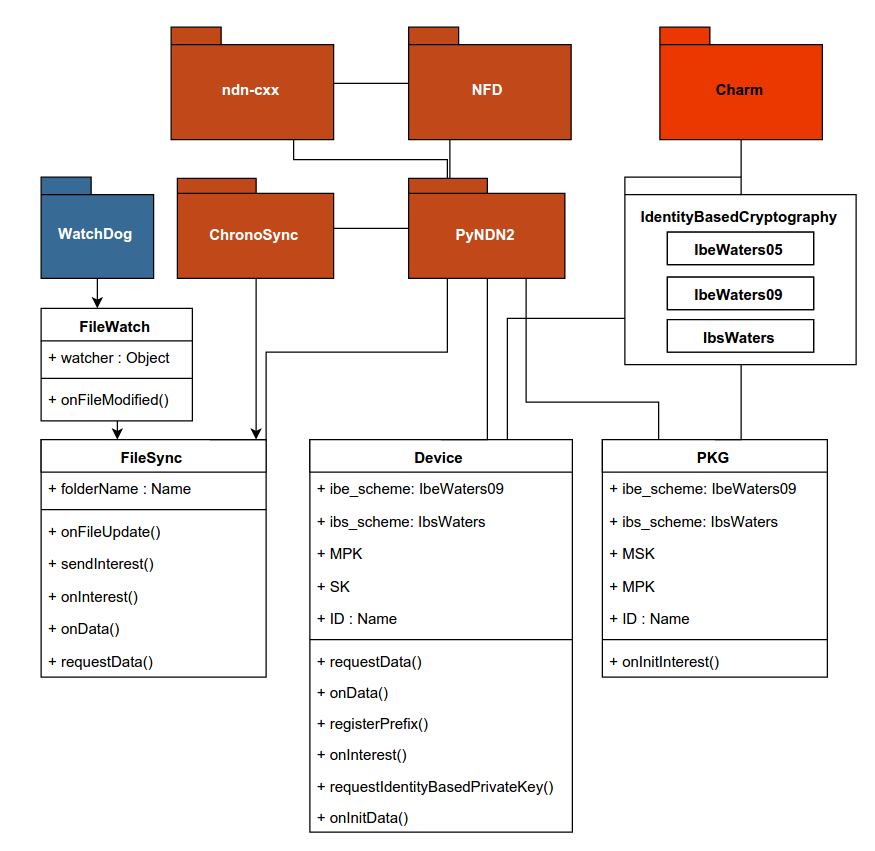
\includegraphics[width=1\textwidth]{code-topology.png}
  \caption{Packages and Classes.}
  \label{fig:code-topology}
\end{figure}

\subsection{Access Control}
In~\autoref{access_control} I present a possible solution for access control.
This is however not implemented in the application, because it is considered too high workload for this thesis.

\subsection{Packet Design}
The packet format is designed with Google Protocol Buffers, which is a language-neutral, platform-neutral, extensible mechanism for serializing structured \gls{data}.\footnote{Google Protocol Buffers - https://developers.google.com/protocol-buffers/}
Initialization packets have the structure presented in~\autoref{fig:init_interest-data}.
Initially the idea was to have the \gls{TMPK} appended to the content \gls{name}. 
However, I experienced a problem where the \texttt{Init} \gls{data} never arrived at destination node. 
After some research in \texttt{ndn-cxx} documentation I found that the packets have a \texttt{MAX\_NDN\_PACKET\_SIZE} of 8800 bytes and the \texttt{Init} \gls{data} exceeded this limit and reached 8904 bytes.
Because the \gls{TMPK} is approximately 2\gls{KB} and was appended to the content \gls{name} in the \gls{interest}, the \gls{data} response off course had to have the same content \gls{name}, hence 2\gls{KB} overhead in the \gls{name}. 
The \gls{TMPK} can as easily be appended to the KeyLocator \gls{name}, hence the \gls{data} response can be 2\gls{KB} less, resulting to a 6866 bytes \texttt{Init} \gls{data} packet.

Sensor packets have the structure presented in~\autoref{fig:sensor_interest-data}.
The code can be reviewed in~\cite[messageBuf.proto]{garseg15}.
\begin{description}
	\item[\texttt{Init} \gls{interest}] - 
  The \texttt{Init} \gls{interest} can be seen in~\autoref{fig:init_interest-data} and consist of three fields: Content Name, KeyLocator and MustBeFresh.
  KeyLocator can be of type \gls{name}. 
  As described in the \gls{NDN} Packet Format~\cite{ndnpacketformat}, generally this field can be used to specify where to download the certificate used to sign the \gls{interest}.
  However, in the trust model I use this field to publish the requesters \gls{name}, i.e. the requesters public key. 
  This is very useful when using \gls{IBE} and \gls{IBS}.
	\item[\texttt{Init} \gls{data}] - 
  The \gls{data} response to the \texttt{Init} \gls{interest} is illustrated in~\autoref{fig:init_interest-data}.
	\item[\texttt{Sensor} \gls{interest}] -
	As in the \texttt{Init} \gls{interest} the KeyLocator field is used to define the ID\textsubscript{requester}. 
  The packet is illustrated in~\autoref{fig:sensor_interest-data}.
	\item[\texttt{Sensor} \gls{data}] - 
  The \gls{data} response to the \texttt{Sensor} \gls{interest} uses the same structure as the \texttt{Init} \gls{data}. 
  It is illustrated in~\autoref{fig:sensor_interest-data}
\end{description}

The \texttt{Init} and \texttt{Sensor} \gls{data} responses in the \gls{HSS} have a structure that is defined in~\cite[messageBuf.proto]{garseg15}.
The fields are:
\begin{itemize}
  \item \texttt{MessageType} is an \texttt{enum} and can be either Init or Sensor.
  \item \texttt{EncAlgorithm} is an \texttt{enum} and represents which type of encryption scheme is used on the content.
  \item \texttt{IbeAlgorithm} is an \texttt{enum} and represents which type of \gls{IBE} scheme is used on the \gls{CEK}.
  \item \texttt{IbsAlgorithm} is an \texttt{enum} and represents which type of \gls{IBS} scheme is used to sign the \gls{data}.
  \item \texttt{MasterPublicKey} is the \gls{PKG}s public parameters used to do \gls{IBE}.
  \item \texttt{SignatureMasterPublicKey} is the \gls{PKG}s public parameters used to do \gls{IBS}.
  \item \texttt{SymmetricKey} is the symmetric key used to encrypt the content. The key is encrypted.
  \item \texttt{Cipher} is the encrypted content.
  \item \texttt{Session} is a nonce.
\end{itemize}

\begin{figure}[ht]
  \centering
  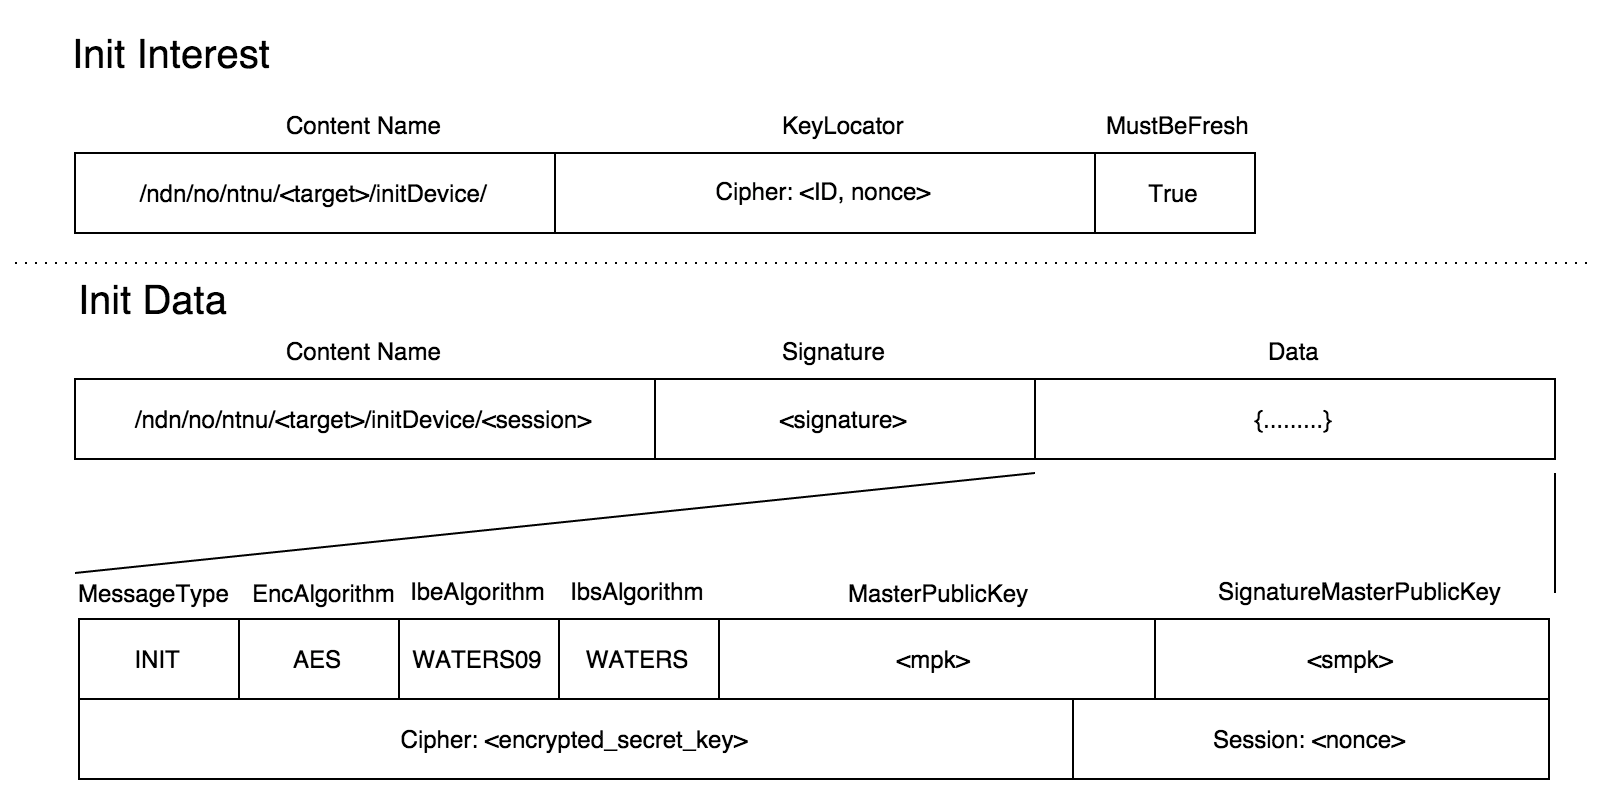
\includegraphics[width=1\textwidth]{init_interest-data.png}
  \caption{Initialization \gls{interest} and \gls{data}}
  \label{fig:init_interest-data}
\end{figure}

\begin{figure}[ht]
  \centering
  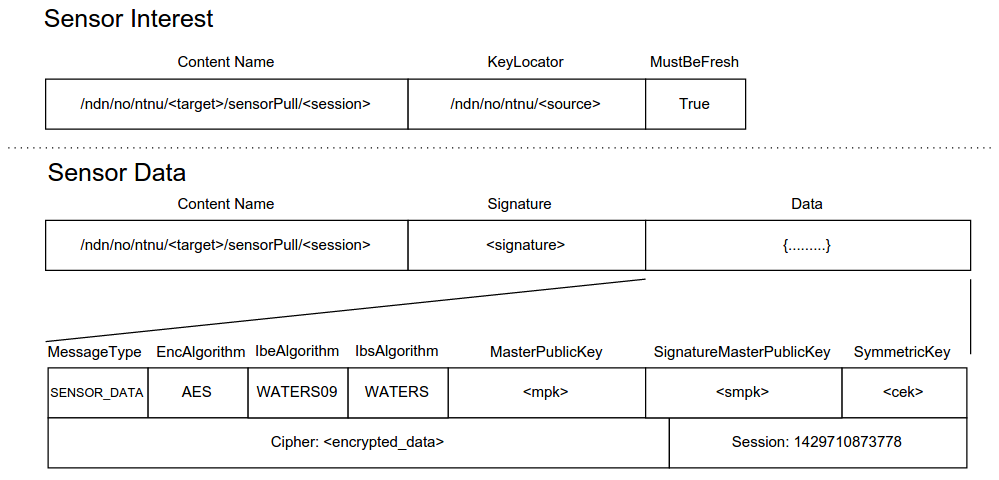
\includegraphics[width=1\textwidth]{sensor_interest-data.png}
  \caption{Sensor \gls{interest} and \gls{data}}
  \label{fig:sensor_interest-data}
\end{figure}

\subsection{Running the Code}
First the \gls{NFD} must be started on each device shown in~\autoref{lst:nfd-start}, if not already running. 
Then we have to make sure that each device participating in the network know the \gls{name} and \gls{IP} address binding, since the testing will run \gls{NDN} over \gls{IP}.
This is accomplished by registering the mapping in the \gls{FIB} at each device showed in the second line in~\autoref{lst:nfd-start}.

On the device playing the role of the \gls{PKG}, run the code presented in~\autoref{lst:pkg}. 
This will create the key pair MPK\textsubscript{pkg} and MSK\textsubscript{pkg} and register the prefix where the other nodes can find the \gls{PKG}.

On the device playing the role of e.g. a sensor, run the code presented in~\autoref{lst:data}.
This will automatically register the prefix of the sensor, and start the initialize protocol with the \gls{PKG}.

On the device playing the role of the user device (e.g. a mobile), run the code presented in~\autoref{lst:pull}.
This will automatically start the initialize protocol with the \gls{PKG}.
Running \texttt{r} will make the device expressing an \gls{interest} for sensor \gls{data} from the sensor.

\begin{lstlisting}[language=bash, caption={NFD Start}, label={lst:nfd-start}]
  $ nfd-start
  $ nfdc register /ndn/no/ntnu/<data-device> udp://<device-ip-address>
  $ nfdc register /ndn/no/ntnu/<pull-device> udp://<device-ip-address>
  $ nfdc register /ndn/no/ntnu/<pkg> udp://<pkg-ip-address>
\end{lstlisting}

\begin{lstlisting}[language=bash, caption={Start PKG}, label={lst:pkg}]
  $ python application.py
  $ pkg
\end{lstlisting}

\begin{lstlisting}[language=bash, caption={Start a device registering a prefix.}, label={lst:data}]
  $ python application.py
  $ data
\end{lstlisting}

\begin{lstlisting}[language=bash, caption={Start a device that will express \gls{interest} in \gls{data}.}, label={lst:pull}]
  $ python application.py
  $ pull
  $ r
\end{lstlisting}

\section{Testing}
In this section it will be presented which computers will be used during testing. 
The measurement results will be presented together with the key/content sizes related to the \gls{HSS}.

\subsection{Computers}
The plan was to test the application with several Raspberry Pi's to simulate a sensor network, with limited computation power.
However this is not possible with the Charm framework as it is not compatible with ARM processors.
The \gls{HSS} is tested over several computers presented in~\autoref{tbl:target_computers}.
Each computer is assigned an ID which will be used for reference in the performance measurements.

\begin{table}[h]
  \begin{tabular}{llll}
  ID      & Computer                  & Operating System          & Processor                    \\ \hline
  C1      & Macbook Pro               & 64-bit OS X 10.10         & Intel Core i7 @ 2.0GHz       \\ %\hline
  C2      & Garsbook                  & 64-bit Ubuntu 14.04 LTS   & Intel Core i5 @ 3.0GHz       \\ %\hline
  C3      & HP                        & 64-bit Ubuntu 14.04 LTS   & Intel Core i7 @ 2.8GHz       \\ %\hline
  \end{tabular}
  \caption{Computers used during tests.}
  \label{tbl:target_computers}
\end{table}

\subsection{Key Sizes}
It is listed in~\autoref{tbl:size_chart} the different sizes for keys related to the \gls{IBE} and \gls{IBS} that is used in the \gls{HSS} implementation.
The \gls{CEK} is generated as a group element and is extracted to 40 bytes when performing encryption and decryption with \gls{AES}.
I would prefer to encrypt and send the extracted version of the \gls{CEK}, i.e. the hash value of 40 bytes, but the \gls{IBE} encryption scheme demands a certain type of format on the \gls{data}, and thus the whole \gls{CEK} must be sent.
The \gls{CEK} is a random $\mathbb{G}_T$ element (\autoref{ibe-secureness}), and is generated with \texttt{group.random(GT)}.
\begin{table}[h]
  \begin{tabular}[c]{p{0.4\textwidth}p{0.2\textwidth}p{0.2\textwidth}}
  Data                            & Scheme          & Size              \\ \hline
  Content Encryption Key (CEK)    & Hash($\mathbb{G}_T$) & 244 bytes         \\ %\hline
  IBE Master Public Key           & Waters09        & 2014 bytes        \\ %\hline
  IBE Secret Key (SK)             & Waters09        & 1164 bytes        \\ %\hline
  IBE Encrypted CEK               & Waters09        & 1472 bytes        \\ %\hline
  Encrypted SK                    & AES             & 1633 bytes        \\ %\hline
  IBS Master Public Key           & Waters          & 2360 bytes        \\ %\hline
  IBS Secret Key (SSK)            & Waters          & 260 bytes         \\ %\hline
  IBS Signature                   & Waters          & 412 bytes         \\ %\hline
  Encrypted SSK                   & AES             & 437 bytes         \\ %\hline
  \end{tabular}
  \caption{Sizes of different keys used in the health sensor system implementation.}
  \label{tbl:size_chart}
\end{table}


\subsection{Performance}\label{ibc-performance}
To be able to evaluate if \gls{IBC} is applicable to devices with small computation power and limited battery, it has to at least perform somewhat in the range of regular asymmetric encryption (read RSA), and signing. 
Naccache suggested that if the prime \gls{p} is 1024-bit, the scheme would provide equivalent security as a RSA 1024-bit key.
For comparison reasons, the RSA key pair is therefore generated with the size of 1024-bit.
In~\autoref{tbl:time_chart} the results from running different cryptographic methods on the computers listed in~\autoref{tbl:target_computers} are presented.

\begin{table}[h]
  \begin{tabular}[c]{lllll}
  Method                                      & Scheme          & C1              & C2          & C3              \\ \hline
  IBE PKG key pair generation                 & Waters09        & 99.65 ms        & 27.09 ms    & 36.08 ms     \\ %\hline
  IBE Encrypting CEK                          & Waters09        & 52.65 ms        & 189.15 ms   & 24.86 ms     \\ %\hline
  IBE Secret Key (SK) generation              & Waters09        & 56.14 ms        & 17.86 ms    & 23.27 ms     \\ %\hline
  Encrypting SK                               & AES             & 0.13 ms         & 0.10 ms     & 0.15 ms     \\ %\hline
  IBS PKG key pair generation                 & Waters          & 97.55 ms        & 27.15 ms    & 35.02 ms     \\ %\hline
  IBS Secret Key (SSK) generation             & Waters          & 9.76 ms         & 2.87 ms     & 3.72 ms     \\ %\hline
  IBS Sign                                    & Waters          & 9.90 ms         & 2.88 ms     & 3.69 ms     \\ %\hline
  IBS Verify                                  & Waters          & 7.58 ms         & 2.66 ms     & 4.32 ms     \\ %\hline
  Encrypting SSK                              & AES             & 0.06 ms         & 0.02 ms     & 0.04 ms     \\ %\hline
  RSA (1024-bit) key pair generation          & RSA             & 254.27 ms       & 119.34 ms   & 165.99 ms     \\ %\hline
  RSA Encryption                              & RSA             & 14.80 ms        & 4.40 ms     & 6.52 ms     \\ %\hline
  RSA Decryption                              & RSA             & 14.72 ms        & 4.45 ms     & 6.49 ms     \\ %\hline
  RSA Sign                                    & RSA             & 16.15 ms        & 4.59 ms     & 6.69 ms     \\ %\hline
  RSA Verify                                  & RSA             & 15.72 ms        & 4.53 ms     & 6.74 ms     \\ %\hline
  ECDSA key pair generation                   & ECDSA           & 0.57 ms         & 0.20 ms     & 0.32 ms     \\ %\hline
  ECDSA Sign                                  & ECDSA           & 0.50 ms         & 0.21 ms     & 0.33 ms     \\ %\hline
  ECDSA Verify                                & ECDSA           & 0.90 ms         & 0.37 ms     & 0.58 ms     \\ %\hline
  \end{tabular}
  \caption{Cryptographic methods time chart. Each measurement is the mean time of 100 rounds and measured in milliseconds. }
  \label{tbl:time_chart}
\end{table}


The initialization protocol described in~\autoref{init} and the data pull protocol described in~\autoref{data_pull} is tested on the computers listed in~\autoref{tbl:target_computers}.
The results of the round trip time are presented in~\autoref{tbl:rtt_chart}.
\begin{table}[h]
  \begin{tabular}[c]{p{0.40\textwidth}p{0.15\textwidth}p{0.15\textwidth}p{0.15\textwidth}}
  Protocol                                & C1            & C1            & C3            \\ \hline
  Initialization                          & 202.9 ms      & 70.8 ms       & 116.3 ms     \\ %\hline
  Data Pull                               & 61.4 ms       & 31.0 ms       & 46.2 ms     \\ %\hline
  \end{tabular}
  \caption{Round trip time chart. Time is measured in milliseconds.}
  \label{tbl:rtt_chart}
\end{table}

The \gls{HSS} is tested on two of the computers in~\autoref{tbl:target_computers}.
The topology is shown in~\autoref{fig:hss-testbed}.
\begin{figure}[ht]
  \centering
  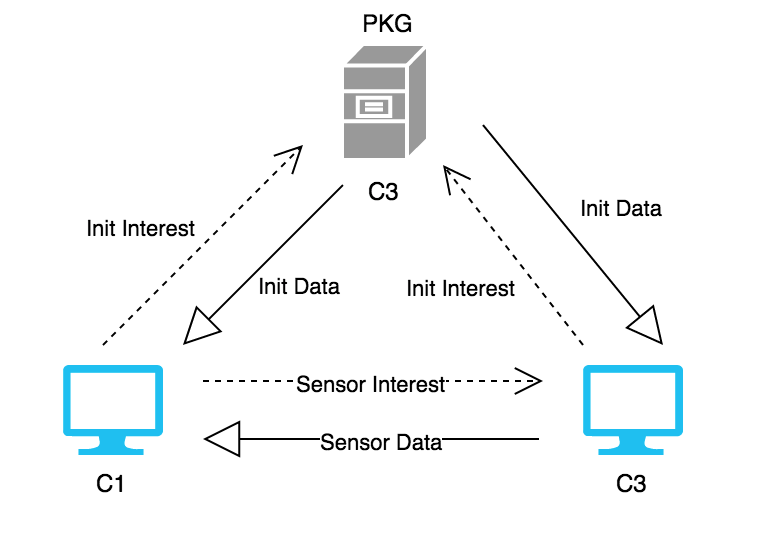
\includegraphics[width=1\textwidth]{hss-testbed.png}
  \caption{Health Sensor System implementation tested over two computer. C3 runs two nodes, i.e. the PKG and one device. C1 runs a second device.}
  \label{fig:hss-testbed}
\end{figure}

\section{NDN Testbed}
The \gls{NDN} testbed is a network of \gls{NDN} nodes created for research purpose. 
\gls{ntnu} joined the testbed contributing with the 24\textsuperscript{th} node in the NDN testbed.
The map of the NDN testbed is shown in~\autoref{fig:ndn-map}.

\begin{figure}[ht]
  \centering
  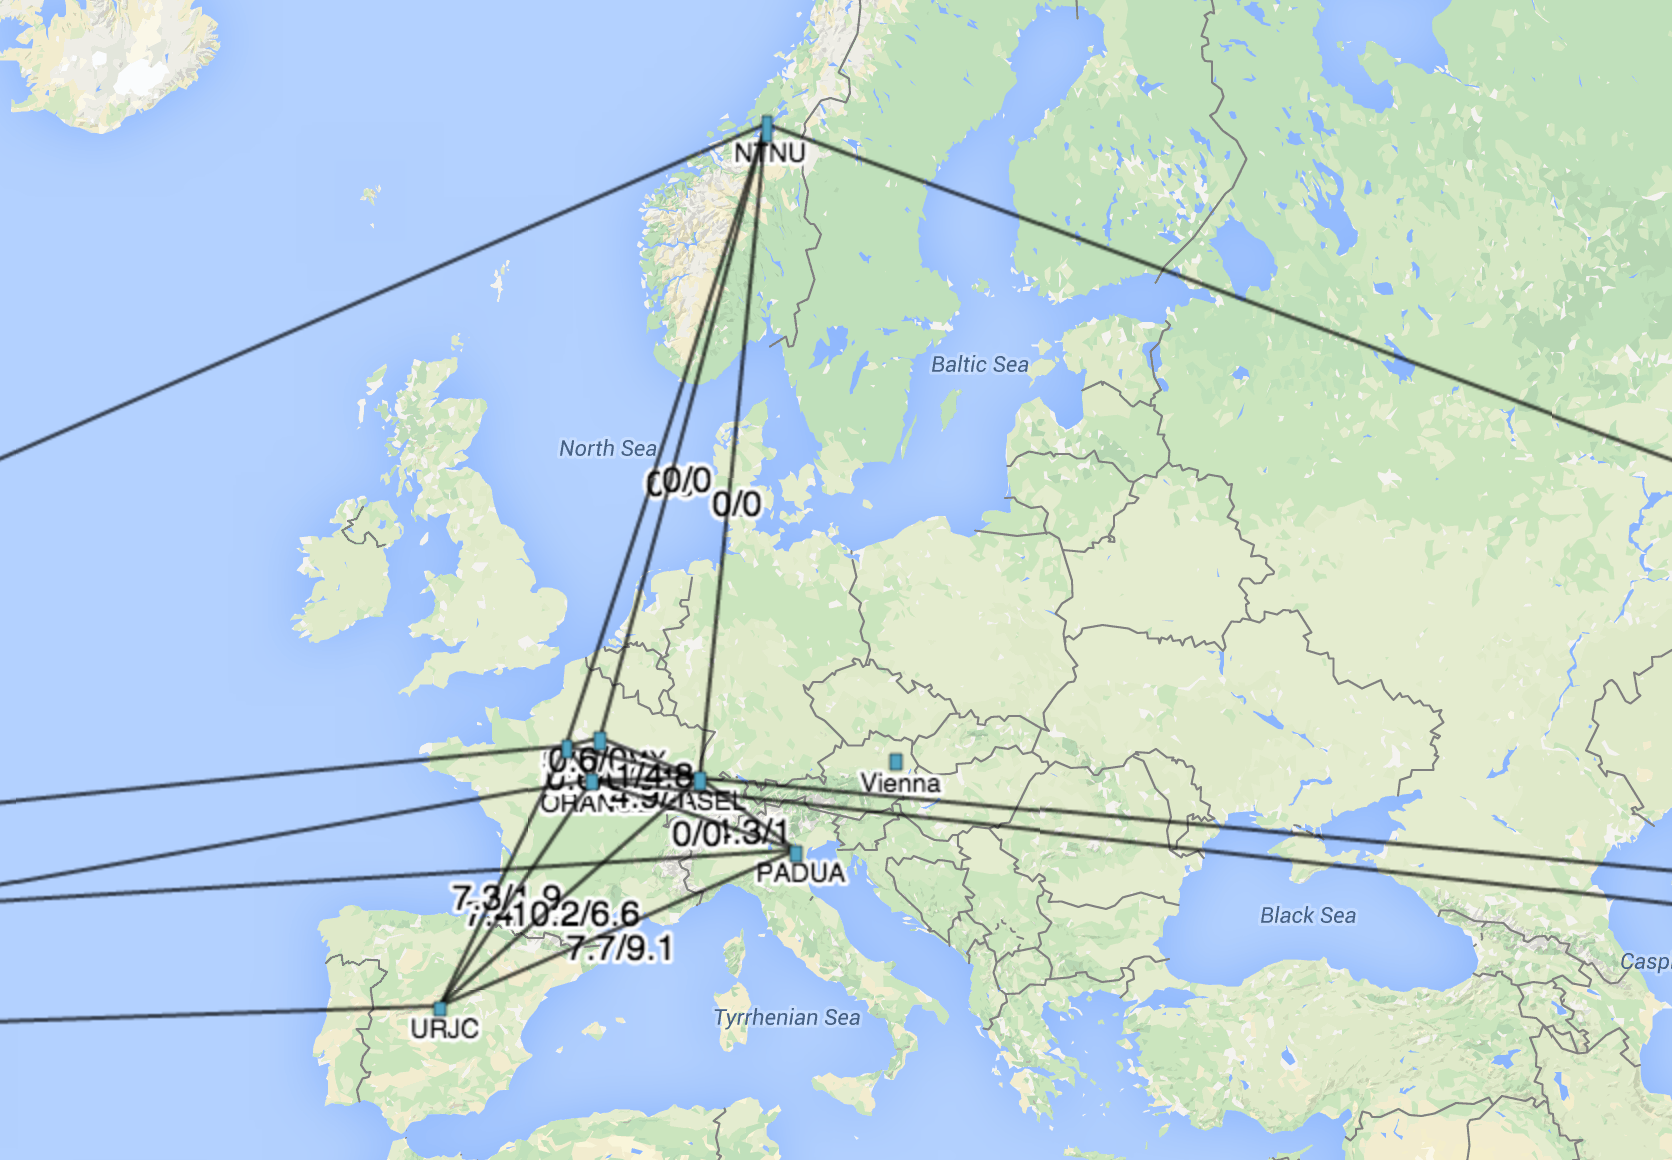
\includegraphics[width=1\textwidth]{ndn-map.png}
  \caption{NDN Testbed Map}
  \label{fig:ndn-map}
\end{figure}

\chapter{Discussion}
In this chapter the work done in conjunction to this thesis will be discussed. 
First I will talk about the pros and cons using \gls{IBC} in \gls{NDN}.
Then I will discuss the \gls{HSS} and possible drawbacks in the system. 
Scalability issues and other applicable networks for the application will be mentioned.

\section{Identity-Based Cryptography in Named Data Networking}
Concerning key revocation, one suggestion has been to add a monthly timestamp to the \gls{name}, but the the \gls{PKG} has to renew private keys for everybody each month. 
This solution do not scale very well due to a lot of computation at the \gls{PKG}.
With the \gls{FSM}, every user will be notified when a identity is revoked.
There is no use for periodically checking names.
But the renewal of keys might not be an issue in the \gls{HSS}. \todo{more..}

\todo{refactor this section}
Can authenticate \gls{data} even using insecure DNS or HTTP. 
There is only one linkage between the \gls{name} and the content, and if the user obtains the right \gls{MPK}, there is no doubt where the \gls{data} originates from and that it is not altered.
In RSA public key cryptography we have to find the key related to the signature. 
In worst case this will be equivalent of retrieving the \gls{MPK} each time, which is not likely. 
Or the \gls{MPK} can be appended to the message.

usability 



\section{Development Usability in Named Data Networking}
Once a basic perception of the \gls{NDN} architecture is understood, it is easy to begin developing.
The \gls{PyNDN2} framework comes with good examples of how to develop simple applications with packets that are signed and encrypted.

The concept of naming \gls{data} introduces more simplicity, but also a new way of application design thinking.
Addressing is dealt with one place in the architecture compared to an equivalent system over \gls{IP}. 
Security is easily applied in \gls{NDN}.

\section{Health Sensor System}
The application is not tested on with real sensors, hence I cannot conclude with anything regarding the computational power of such devices, nor the life time of the battery when performing \gls{IBE}.  

Power efficiency
\todo{more on this}

A problem with \gls{wsn} in \gls{IP} networks, is that it is a limited number of \gls{IP} adderesses (especially in \gls{IPv4}).
So the global scalability issue arises due to the potentially large number of sensors that could be deployed. 
With the naming rules in \gls{NDN}, this is not a issue.

In~\autoref{ibc-performance} we can see that \gls{IBC} is performing better than regular asymmetric cryptography, RSA. 

Encrypting with same symmetric key for each set of \gls{data}, limits the encryption computation for the device if several devices requests the same \gls{data}.
Using a unique key for each time \gls{data} is requested is more secure and can be used for more sensitive content.

Who can play the role of a device?
As mentioned in~\autoref{rendezvous_authentication} and~\autoref{init} there should be a limitation of which devices that can be initialized to the trust domain.
\todo{hm... something here?}

Storing the \gls{SK} in a secure fashion.

Preloading secret key, offline mode, yet the initialization protocol should be used to do this, unless the sharing is done in a wired environment. 
\gls{NFC} signal is hard (impossible?) to eavesdrop, thus the initialization protocol is not needed. 


\section{Scalability}
Distributing the \gls{ID}-list can be an issue, as the list can grow linearly with the number of participants in the trust domain.
However, this might not be a huge problem in the use cases that is addressed in this thesis, considering that the number of devices in the \gls{HSS} will not grow larger than e.g. 100 devices. 

\section{Sync}
The sync application makes it possible for users to know who has a valid public key within the \gls{PKG}s domain.
One drawback with the key distribution using \gls{FSM} is that for the sender to be 100\% sure that the message is encrypted with the latest \gls{ID}, the sender has to rely on that it has received the latest sync state available from the \gls{PKG}.
Likewise when a \gls{receiver} verifies a signature, it has to rely on the same principle to be able to know if the belonging \gls{ID} is still valid.
Since the scalability is not that big of an issue in this scenario, the monthly (or even more often) timestamp appended to the \gls{ID} might be a good solution to reduce the time of exposure when compromised.

There are some issues that could occur in such a system. 
\gls{DoS} on Sync \gls{interest} and Sync \gls{data}. 
If the \gls{FSM} is used to revoke public keys as suggested, an attacker who has found the compromised \gls{SK}, can try to deny the distribution of the new list, i.e. the Sync \gls{data}, from the distributor. 
This is however a complicated attack and an updated list would spread fast.
Performing \gls{DoS} on every node is not easy, and would block the network access for the adversary anyway.
In~\cite{DBLP:conf/spw/StajanoA99} Frank Stajano and Ross Anderson mentions possible \gls{DoS} attacks, such as radio jamming and battery exhaustion. 
All applications that relies on some sort of crucial information derived using \gls{FSM} (\autoref{file-sync}) are vulnerable to this kind of \gls{DoS}.

\section{Other Use Cases}
The trust model used in the \gls{HSS} can be used in any network where the use of a \gls{TTP} is accepted. 
Such a system can for instance be:
\begin{enumerate}
	\item Home automation systems
	\item \gls{BAS}
	\item \gls{BMS}
	\item Health care
	\item Military networks
	\item Sensor networks such as disaster, habitat and hazard monitoring
\end{enumerate}



\chapter{Conclusion and Future Work}\label{chp7:conclusion}
%\chapter{NDN node 23 - NTNU}

\section{NDN node 23 - NTNU}
Node 23 in NDN testbed

\begin{figure}[ht]
  \centering
  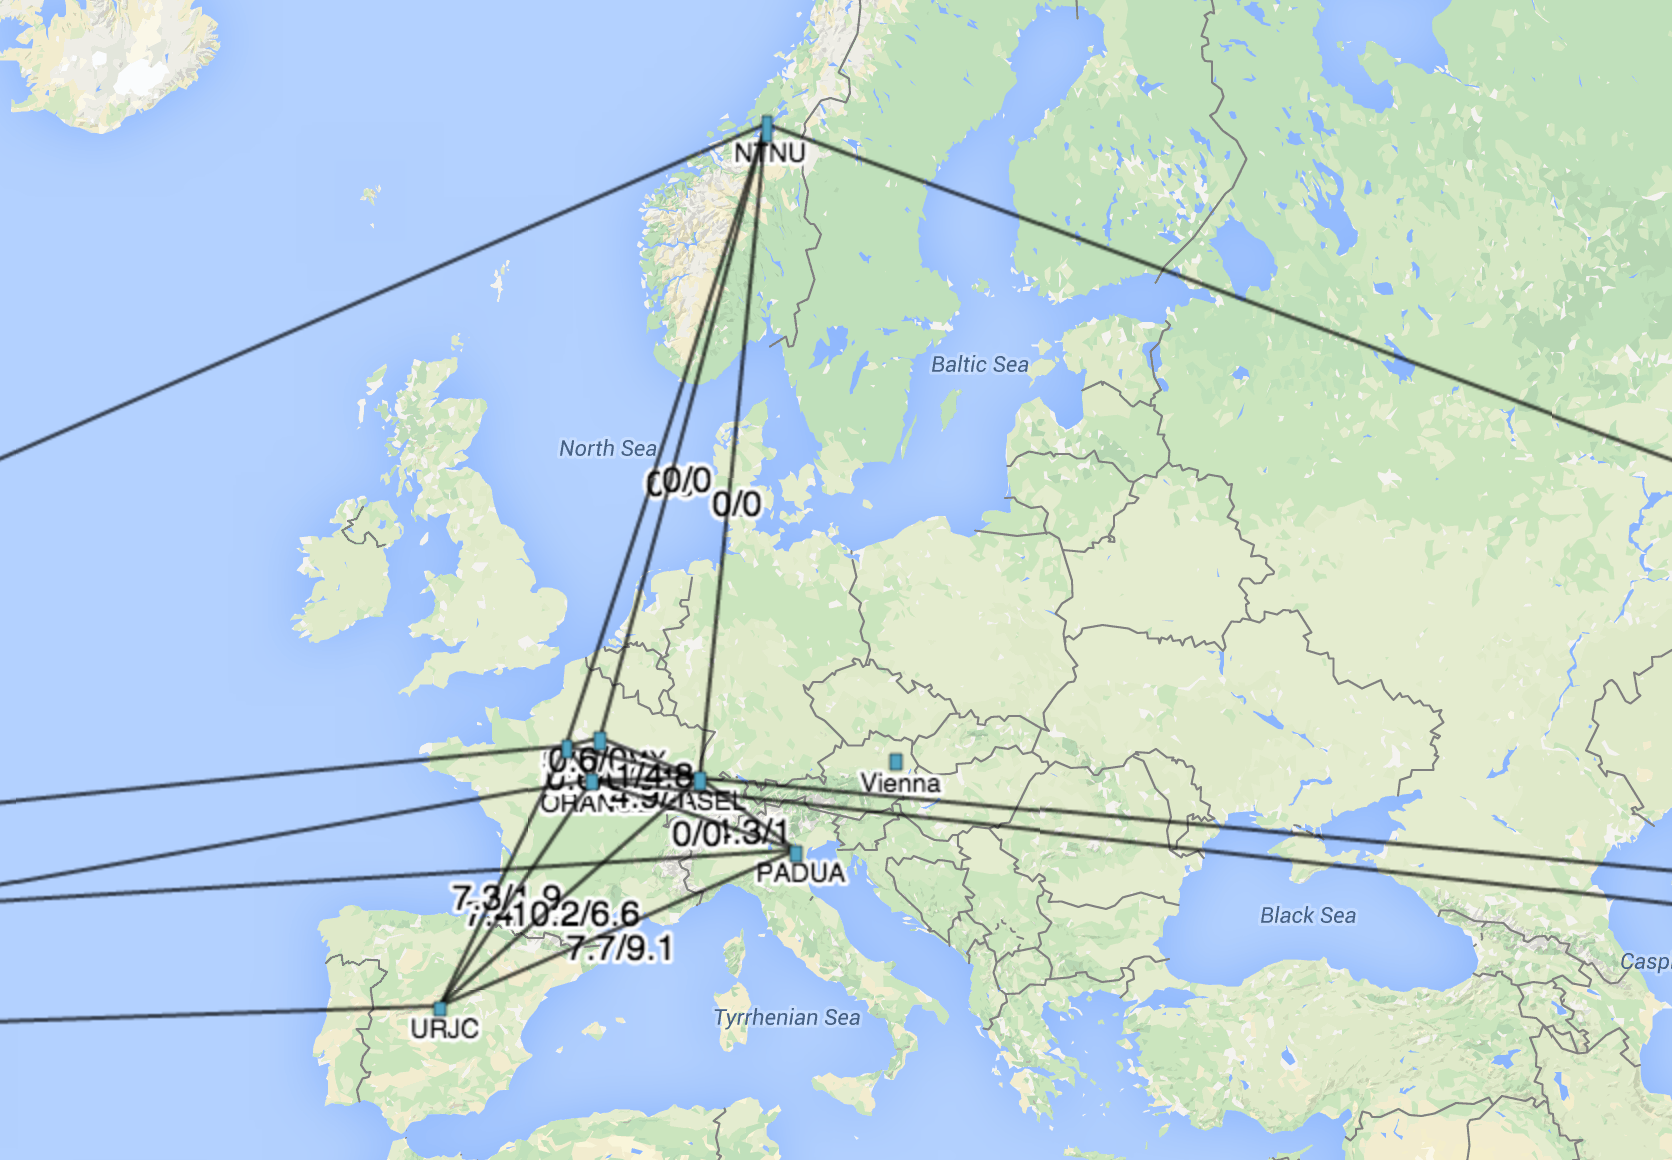
\includegraphics[width=1\textwidth]{ndn-map.png}
  \caption{NDN Map}
  \label{fig:ndn-map}
\end{figure}

%% include here the other chapters

%% References
%\include{references}
\renewcommand*{\bibname}{References}
%\bibliographystyle{ieeetr}
\bibliographystyle{alpha}
\bibliography{main}

% Uncomment the following if you have any appendix
\appendix
\addtocontents{toc}{%
 \protect\vspace{1em}%
 \protect\noindent \bfseries \appendixtocname\protect\par
 \protect\vspace{-.5em}%
}
\renewcommand{\chaptername}{\appendixname}
% include below possible appendices (chapters)
%\include{appendix}
\chapter{ChronoSync}\label{apx:chronosync}

Since \gls{NDN} provides multicast in the network layer as explained in~\autoref{fig:ndn-multicast}, we do not have to think of network load in the same way as in \gls{IP}.  
To achieve distributed synchronization of a \gls{data}set, the \gls{NDN}-team has developed ChronoSync, a decentralized synchronization framework over \gls{NDN}. 
ChronoSync assumes that a group of nodes knows the \gls{name} of a \gls{synchronization_group}, e.g \path{/ndn/broadcast/FileSync-0.1/<group_room>/}.
The synchronication application is built upon state digests, which is that each participating node stores a hash of its current \gls{data}set. 
Each node in a ChronoSync application broadcasts its sync state in a Sync \gls{interest} (e.g. \path{/ndn/broadcast/FileSync-0.1/<group_room>/<state>}).
When a node receives a Sync \gls{interest}, it will inspect the state of the \gls{interest}, and compare with its own state.
Each node holds a state tree that is used to detect new and outdated states.
If the incoming \gls{interest} state is equal to the receiving node's state, the node has no reason to do anything, as the system is in a \textit{stable state} from the node's point of view.
If not, the receiving node has to find out whether the incoming \gls{interest} is 1) a state the node itself has been in, or if its 2) a new state.
In case of 1), the receiving node has new \gls{data} and should provide the new content as a response to the incoming \gls{interest}. In case of 2), the receiving node should send out a Recovery \gls{interest} for the new state.

\begin{enumerate}
  \item \textit{Sync \gls{interest}} is an \gls{interest} that a participating node sends out to discover new \gls{data}.
  \item \textit{Sync \gls{data}} is a response to 1), if a participating node has new \gls{data}.
  \item \textit{Recovery \gls{interest}} is an \gls{interest} sent out if a node discovers that another node has a newer state.
  \item \textit{Recovery \gls{data}} is a response to 3).
\end{enumerate}

When the group is in a stable state, each Sync \gls{interest} is equivalent, hence only one entry at each router's \gls{PIT} is created, forming a temporary multicast three.
This \gls{interest} is periodically sent out from each subscriber maintaining the multicast three, resulting in that the producer has the possibility to answer the Sync \gls{interest} with Sync \gls{data} whenever the producer has a new \gls{data}set.

ChronoSync is only taking care of \gls{data} discovery, and leaves other logic to the application that is using ChronoSync. 
Such logic can be e.g. what should happen when a new participant enters the room.
Should all history be downloaded? 
Or who is allowed to publish content in each \gls{synchronization_group}?

ChronoSync is explained in detail here~\cite{DBLP:conf/icnp/ZhuA13}.
\chapter{Code}\label{apx:code}

\lstset{language=Python, 
    basicstyle=\ttfamily\small, 
    keywordstyle=\color{keywords},
    commentstyle=\color{comments},
    stringstyle=\color{red},
    showstringspaces=false,
    %procnamekeys={def,class}
    identifierstyle=\color{green}
    }

\section{Scyther Security Analysis of Device Registration}\label{apx:scyther-analysis-dr}
To better understand the code,~\autoref{tbl:mapping_code} is presents mapping of the~\autoref{fig:init_ibe_2} to the code.

\begin{table}[h]
  \begin{tabular}{lll}
  Figure      				& SPDL Code     			& Description 				\\ \hline
  ID\textsubscript{d}  		& D   						& Identity of the device 	\\ %\hline
  ID\textsubscript{PKG}   	& PKG      					& Identity of the PKG 		\\ %\hline
  n      					& R            				& Random nonce 				\\ %\hline
  sk      					& SK           				& Secret key to an identity	\\ %\hline
  c\textsubscript{1} = AES\_Enc\textsubscript{tk}[ID\textsubscript{d} || n]  & c1 = \{ D, R \}k(PKG,D)   & AES encrypted content		\\ %\hline
  c\textsubscript{2} = AES\_Enc\textsubscript{tk}[sk || \~{n}]     	& c2 = \{ SK, R \}k(PKG,D)	& AES encrypted content 	\\ %\hline
  s = Sign(mpk || sk\textsubscript{pkg} || c\textsubscript{2})      & s = \{ SHA1(c2) \}sk(PKG)   & Signature				\\ %\hline
  \end{tabular}
  \caption{Mapping of the~\autoref{fig:init_ibe_2} and the \gls{spdl} code.}
  \label{tbl:mapping_code}
\end{table}

\begin{lstinputlisting}
[language=Python]{../src/device_registration.spdl}
\end{lstinputlisting}

\clearpage
\section{Scyther Security Analysis of Data Pull}\label{apx:scyther-analysis-dp}
To better understand the code,~\autoref{tbl:mapping_code_data} is presents mapping of the~\autoref{fig:data_pull_ibe} to the code.

\begin{table}[h]
  \begin{tabular}{lll}
  Figure      				& SPDL Code     			& Description 				\\ \hline
  ID\textsubscript{d}  		& D   						& Identity of the device 	\\ %\hline
  ID\textsubscript{m}   	& M      					& Identity of the mobile	\\ %\hline
  n      					& R            				& Random nonce 				\\ %\hline
  sk      					& SK           				& Secret key to an identity	\\ %\hline
  c\_cek = Encrypt(mpk || ID\textsubscript{d} || cek)	& ccek = \{ cek \}pk(D) 		& IBEncrypted CEK 	\\
  c = AES\_Enc\textsubscript{cek}(data || \~{n}) 		& c = \{ data , R \}k(M,D) 	& AES encrypted content 	\\
  m\textsubscript{1} = (ID\textsubscript{d} || n || request)  & m1 = (M, D, R)   	& Message		\\ %\hline
  c\textsubscript{2} = (c\_cek || c)     	& c2 = (M, c, ccek)						& Message 	\\ %\hline
  s\textsubscript{1} = Sign(mpk || sk\textsubscript{m} || c\textsubscript{1})      	& s1 = { SHA1(m1) }sk(M)   & Signature				\\ %\hline
  s\textsubscript{2} = Sign(mpk || sk\textsubscript{d} || c\textsubscript{2}      	& s2 = { SHA1(c2) }sk(D)   & Signature				\\ %\hline
  \end{tabular}
  \caption{Mapping of the~\autoref{fig:init_ibe_2} and the \gls{spdl} code.}
  \label{tbl:mapping_code_data}
\end{table}

\begin{lstinputlisting}
[language=Python]{../src/data_pull.spdl}
\end{lstinputlisting}

% \section{File Sync}\label{apx:file-sync-code}

% Using watchdog to observe files

% \begin{lstinputlisting}
% [language=Python]{../../master-thesis-work/fileSync.py}
% \end{lstinputlisting}

% \section{Device}\label{apx:device-code}

% Device, e.g. a sensro device or a mobile.

% \begin{lstinputlisting}
% [language=Python]{../../master-thesis-work/device.py}
% \end{lstinputlisting}

% \section{Public Key Generator}\label{apx:pkg-code}

% \gls{PKG}

% \begin{lstinputlisting}
% [language=Python]{../../master-thesis-work/publicKeyGenerator.py}
% \end{lstinputlisting}

% \section{Identity-Based Encryption}\label{apx:ibe-code}

% \gls{IBE}

% \begin{lstinputlisting}
% [language=Python]{../../master-thesis-work/identityBasedCrypto.py}
% \end{lstinputlisting}

% \section{Main}\label{apx:main-code}

% Main..

% \begin{lstinputlisting}
% [language=Python]{../../master-thesis-work/application.py}
% \end{lstinputlisting}

% \section{Message Buffer Protocol}\label{apx:msgBuf-code}
% \begin{lstinputlisting}
% [language=XML]{../../master-thesis-work/messageBuf.proto}
% \end{lstinputlisting}

\end{document} 
